% XeLaTeX can use any Mac OS X font. See the setromanfont command below.
% Input to XeLaTeX is full Unicode, so Unicode characters can be typed directly into the source.

% The next lines tell TeXShop to typeset with xelatex, and to open and save the source with Unicode encoding.

%!TEX TS-program = xelatex
%!TEX encoding = UTF-8 Unicode

\documentclass[11pt,twoside,openany]{book}
\usepackage{multirow}
\usepackage{pdfpages}

\usepackage{xspace}

\usepackage{array}
\usepackage{lipsum}

\usepackage{algorithm}
\usepackage{algpseudocode}

\usepackage{geometry}                % See geometry.pdf to learn the layout options. There are lots.
%\usepackage[margin=1cm]{geometry}


% \addtolength{\textwidth}{1.75in}
%
% \addtolength{\topmargin}{-.875in}
% \addtolength{\textheight}{1.75in}

\geometry{a4paper,left=20mm,top=20mm,bottom=50mm,total={162mm,230mm}}                   % ... or a4paper or a5paper or ...
%\geometry{landscape}                % Activate for for rotated page geometry
%\usepackage[parfill]{parskip}    % Activate to begin paragraphs with an empty line rather than an indent
\usepackage{amssymb}
%\usepackage{todonotes}
\setlength{\marginparwidth}{2cm}
\usepackage[backgroundcolor=white,bordercolor=blue,linecolor=blue,textwidth=1cm]{todonotes}
\usepackage{booktabs}
\usepackage{longtable}
\usepackage{url}

\usepackage[depth=4]{bookmark}


\usepackage{algorithm}
\usepackage{algpseudocode}

\usepackage{imakeidx}
\usepackage[utf8]{inputenc}
\usepackage[T1]{fontenc}
\makeindex[intoc]

\usepackage[font=normalsize]{caption}

\renewcommand{\theparagraph}{\S\arabic{paragraph}}
\setcounter{secnumdepth}{4}


\usepackage{xcolor}
\usepackage{listings}

\makeatletter
\global\let\tikz@ensure@dollar@catcode=\relax
\makeatother

\definecolor{mGreen}{rgb}{0,0.6,0}
\definecolor{mGray}{rgb}{0.5,0.5,0.5}
\definecolor{mPurple}{rgb}{0.58,0,0.82}
\definecolor{backgroundColour}{rgb}{0.95,0.95,0.92}
\definecolor{gray}{rgb}{0.4,0.4,0.4}
\definecolor{darkblue}{rgb}{0.0,0.0,0.6}
\definecolor{cyan}{rgb}{0.0,0.6,0.6}

\lstdefinestyle{CStyle}{
    backgroundcolor=\color{backgroundColour},
    commentstyle=\color{mGreen},
    keywordstyle=\color{magenta},
    numberstyle=\tiny\color{mGray},
    stringstyle=\color{mPurple},
    basicstyle=\scriptsize\ttfamily,
    breakatwhitespace=false,
    breaklines=true,
    captionpos=b,
    keepspaces=true,
    numbers=left,
    numbersep=5pt,
    showspaces=false,
    showstringspaces=false,
    showtabs=false,
    tabsize=2,
    language=C
}


\lstset{
  backgroundcolor=\color{white},   % choose the background color; you must add \usepackage{color} or \usepackage{xcolor}; should come as last argument
  basicstyle=\footnotesize\ttfamily,        % the size of the fonts that are used for the code
  breakatwhitespace=false,         % sets if automatic breaks should only happen at whitespace
  breaklines=true,                 % sets automatic line breaking
  captionpos=b,                    % sets the caption-position to bottom
  commentstyle=\color{gray},    % comment style
  deletekeywords={...},            % if you want to delete keywords from the given language
  %escapeinside={\%*}{*)},          % if you want to add LaTeX within your code
  %extendedchars=true,              % lets you use non-ASCII characters; for 8-bits encodings only, does not work with UTF-8
  %firstnumber=1000,                % start line enumeration with line 1000
  frame=single,                    % adds a frame around the code
  keepspaces=true,                 % keeps spaces in text, useful for keeping indentation of code (possibly needs columns=flexible)
  keywordstyle=\color{blue},       % keyword style
  language=C,                 % the language of the code
  %morekeywords={*,...},            % if you want to add more keywords to the set
  numbers=left,                    % where to put the line-numbers; possible values are (none, left, right)
  numbersep=5pt,                   % how far the line-numbers are from the code
  numberstyle=\tiny\color{gray}, % the style that is used for the line-numbers
  rulecolor=\color{black},         % if not set, the frame-color may be changed on line-breaks within not-black text (e.g. comments (green here))
  showspaces=false,                % show spaces everywhere adding particular underscores; it overrides 'showstringspaces'
  showstringspaces=false,          % underline spaces within strings only
  showtabs=false,                  % show tabs within strings adding particular underscores
  stepnumber=1,                    % the step between two line-numbers. If it's 1, each line will be numbered
  stringstyle=\color{black},     % string literal style
  tabsize=2,                     % sets default tabsize to 2 spaces
}

\lstset{
  columns=fullflexible,
  showstringspaces=false,
  commentstyle=\color{gray}\upshape,
  backgroundcolor=\color{backgroundColour},
  commentstyle=\color{mGreen},
  keywordstyle=\color{magenta},
  numberstyle=\tiny\color{mGray},
  stringstyle=\color{mPurple},
  basicstyle=\scriptsize\ttfamily,
  tabsize=2
}

\lstdefinelanguage{XML}
{
  morestring=[b]",
  morestring=[s]{>}{<},
  morecomment=[s]{<?}{?>},
  stringstyle=\color{black},
  identifierstyle=\color{darkblue},
  keywordstyle=\color{cyan},
  morekeywords={xmlns,version,type}% list your attributes here
}


% Will Robertson's fontspec.sty can be used to simplify font choices.
% To experiment, open /Applications/Font Book to examine the fonts provided on Mac OS X,
% and change "Hoefler Text" to any of these choices.

\usepackage{fontspec,xltxtra,xunicode}
\defaultfontfeatures{Mapping=tex-text}
\setromanfont[Mapping=tex-text]{Optima}
\setsansfont[Scale=MatchLowercase,Mapping=tex-text]{Optima}
\setmonofont[Scale=MatchLowercase]{Andale Mono}

%%%% Graphics
\usepackage{graphicx}
\usepackage{tikz}
\definecolor{unilublue}{RGB}{55,149,218}
\definecolor{sntred}{RGB}{219,46,27}
\definecolor{sntpurple}{RGB}{86,30,130}
%\definecolor{sntblue}{RGB}{50,130,207}
\definecolor{sntblue}{RGB}{55,149,218}

\pgfdeclareimage[width=30mm]{logo-snt}{logos/logo-snt}
\pgfdeclareimage[width=30mm]{logo-uni-lu}{logos/logo-uni-lu}

%%%% Fancy
\usepackage{fancyhdr}

%%%% Increase page length
\addtolength{\textheight}{1in}

%%%% Sections
\usepackage{sectsty}
\allsectionsfont{\sffamily}

\setlength{\parskip}{1em}

%\renewcommand{\,}{$^{\cdot}$}

\usepackage{hyperref}
\hypersetup{
    colorlinks,
    citecolor=black,
    filecolor=black,
    linkcolor=black,
    urlcolor=black
}


%%%% Title
\newcommand{\titleone}{\textsf{FAQAS Framework}}
\newcommand{\titletwo}{\textsf{SUM}}
\newcommand{\titlethree}{\textsf{Software User Manual}}

\newcommand{\todoinline}[1]{\todo[color=orange,inline]{ \textbf{TODO}: #1 }}

\newcommand{\TODO}[1]{\todo[color=orange,inline]{ \textbf{TODO}: #1 }}
\newcommand{\OSCAR}[1]{\todo[color=yellow,inline]{ \textbf{OSCAR}: #1 }}
\newcommand{\DONE}[1]{\todo[color=green,inline]{ \textbf{DONE}: #1 }}

\newcommand{\CHANGEDTWO}[1]{\textcolor{black}{#1}}

\newcommand{\EMPH}[1]{\textbf{\emph{#1}}}
\newcommand{\INDEX}[1]{\index{\MakeLowercase{#1}}\EMPH{#1}}

\newcommand{\MASS}{\textit{MASS}\xspace}

\newcommand{\DAMA}{\textit{DAMAt}\xspace}

\newcommand{\SEMU}{\textit{SEMu}\xspace}

\newcommand{\SEMUS}{\textit{SEMuS}\xspace}

\newcounter{paranum}
\newcommand{\RQ}{\vspace{10pt}\noindent\textbf{FAQAS-SSS-REQ-\refstepcounter{paranum}\ifnum\value{paranum}<10 00\else 0\fi\theparanum}\textbf}

\newcommand{\remark}{\textbf{Remark:}\xspace}

\begin{document}

\pagestyle{fancy}
\renewcommand{\sectionmark}[1]{\markright{\textit{#1}}}

\renewcommand{\headrulewidth}{2pt}% 2pt header rule
\renewcommand{\headrule}{\hbox to\headwidth{%
  \color{sntblue}\leaders\hrule height \headrulewidth\hfill}}

\fancyhf{}

%\lhead{\fancyplain{}{\setlength{\unitlength}{1mm}
%\begin{picture}(0,0)
%\put(0,-4){
\includegraphics[width=50pt]{logos/logo-snt}}
%\end{picture}}}

\lhead{\fancyplain{}{\textit{}}}

\rhead{\fancyplain{}{\rightmark }}

\fancyfoot[C]{%
\begin{tikzpicture}[remember picture,overlay]
\path [fill=sntred]    ([xshift=88pt,yshift=20pt]current page.south west) rectangle
                       ([xshift=229pt,yshift=50pt] current page.south west);
\path [fill=sntpurple] ([xshift=229pt,yshift=20pt] current page.south west) rectangle
                       ([xshift=370pt,yshift=50pt] current page.south west);
\path [fill=sntblue]   ([xshift=370pt,yshift=20pt] current page.south west) rectangle
                       ([xshift=510pt,yshift=50pt] current page.south west);
\end{tikzpicture}
}

\fancyfoot[RO]{
\begin{tikzpicture}[remember picture,overlay]
\node [circle, ultra thick, fill=white, draw=sntblue] at ([xshift=530pt,yshift=35pt] current page.south west) {\thepage};
\end{tikzpicture}}

\fancyfoot[LE]{
\begin{tikzpicture}[remember picture,overlay]
\node [circle, ultra thick, fill=white, draw=sntblue] at ([xshift=65pt,yshift=35pt] current page.south west) {\thepage};
\end{tikzpicture}}


\newcommand{\STARTCHANGEDWPT}{\color{blue}}
\newcommand{\ENDCHANGEDWPT}{\color{black}}

\newcommand{\CHANGED}[1]{{#1}}
\newcommand{\prog}{P}
\newcommand{\prop}{}

\newcommand{\FAQAS}{FAQAS-framework\xspace}

%\newcommand{\REVISION}[2]{\todo{\tiny{#1}}\color{blue}{#2}\color{black}}
\newcommand{\REVISION}[2]{{#2}}

\newcommand{\REVTWO}[2]{#2}

\thispagestyle{empty}

\begin{tikzpicture}[remember picture,overlay]
\path [fill=sntred]    ([xshift=30pt,yshift=20pt]current page.south west) rectangle
                       ([xshift=210pt,yshift=50pt] current page.south west);
\path [fill=sntpurple] ([xshift=210pt,yshift=20pt] current page.south west) rectangle
                       ([xshift=390pt,yshift=50pt] current page.south west);
\path [fill=sntblue]   ([xshift=390pt,yshift=20pt] current page.south west) rectangle
                       ([xshift=570pt,yshift=51pt] current page.south west);
\path [fill=unilublue] ([xshift=30pt,yshift= 50pt] current page.south west) --
                       ([xshift=570pt,yshift= 50pt] current page.south west)
                       [rounded corners=20pt] --
                       ([xshift=570pt,yshift=740pt] current page.south west)
                       [sharp corners] --
                       ([xshift=30pt,yshift=740pt] current page.south west);
\node [fill=white,rounded corners=0pt,inner xsep=6pt,inner ysep=3pt]
      at ([xshift=523pt,yshift=120pt] current page.south west)
      {\pgfuseimage{logo-uni-lu}};

\node [fill=white,rounded corners=2pt,inner xsep=6pt,inner ysep=3pt]
      at ([xshift=520pt,yshift=780pt] current page.south west)
      {\pgfuseimage{logo-snt}};

%\node [circle, fill=white, draw=sntblue] at ([xshift=550pt,yshift=35pt] current page.south west) {a};

\node[draw=none,fill=none,right] at (-1, -7){\color{white}\LARGE\bf\titleone};
\node[draw=none,fill=none,right] at (-1, -8){\color{white}\LARGE\bf\titletwo};
\node[draw=none,fill=none,right] at (-1, -9){\color{white}\LARGE\bf\titlethree};

\node[draw=none,fill=none,right] at (-1, -12){\color{white}\Large\textsf{O. Cornejo, F. Pastore, E. Viganò}};
\node[draw=none,fill=none,right] at (-1, -13){\color{white}\Large\textsf{Interdisciplinary Centre for Security, Reliability and Trust}};
\node[draw=none,fill=none,right] at (-1, -14){\color{white}\Large\textsf{University of Luxembourg}};
\node[draw=none,fill=none,right] at (11, -16){\color{white}\textsf{ITT-1-9873-ESA-FAQAS-SUTP}};
\node[draw=none,fill=none,right] at (11, -17){\color{white}\Large\textsf{Issue 4, Rev. 1}};
\node[draw=none,fill=none,right] at (11, -18){\color{white}\Large\textsf{\today}};
\node[draw=none,fill=none,right] at (-1, -24){\color{white}\tiny\textsf{EUROPEAN SPACE AGENCY. CONTRACT REPORT.}};
\node[draw=none,fill=none,right] at (-1, -24.3){\color{white}\tiny\textsf{The work described in this report was done under ESA contract. Responsibility for the contents resides in the author or organisation that prepared it.}};
\node[draw=none,fill=none,right] at (-1, -24.8){\color{white}\tiny\textsf{The copyright in this document is vested in the University of Luxembourg.}};
\node[draw=none,fill=none,right] at (-1, -25.1){\color{white}\tiny\textsf{This document may only be reproduced in whole or in part, or stored in a retrieval system,or transmitted in any form, or by any means electronic,}};
\node[draw=none,fill=none,right] at (-1, -25.4){\color{white}\tiny\textsf{mechanical, photocopying or otherwise, either with the prior permission of the University of Luxembourg or in accordance with the terms of ESTEC Contract No. 4000128969/19/NL/AS.}};

\node[draw=none,fill=none,right] at (-1, -24){\color{white}\tiny\textsf{EUROPEAN SPACE AGENCY. CONTRACT REPORT.}}; 
\node[draw=none,fill=none,right] at (-1, -24.3){\color{white}\tiny\textsf{The work described in this report was done under ESA contract. Responsibility for the contents resides in the author or organisation that prepared it.}};
\node[draw=none,fill=none,right] at (-1, -24.8){\color{white}\tiny\textsf{The copyright in this document is vested in the University of Luxembourg.}};
\node[draw=none,fill=none,right] at (-1, -25.1){\color{white}\tiny\textsf{This document may only be reproduced in whole or in part, or stored in a retrieval system,or transmitted in any form, or by any means electronic,}}; 
\node[draw=none,fill=none,right] at (-1, -25.4){\color{white}\tiny\textsf{mechanical, photocopying or otherwise, either with the prior permission of the University of Luxembourg or in accordance with the terms of ESTEC Contract No. 4000128969/19/NL/AS.}};


\end{tikzpicture}

\newpage


% !TEX root = MAIN.tex

\section*{Revisions}
\label{sec:revisions}


\setlength\LTleft{0pt}
\setlength\LTright{0pt}
\tiny 
%@{\extracolsep{\fill}}
\begin{longtable}{|p{2cm}|p{1cm}|p{1.5cm}|p{9cm}|@{}}
\label{table:codeoperators} \\
\hline
\textbf{Issue Number}&\textbf{Date}&\textbf{Authors}&\textbf{Description}\\
\hline
ITT-1-9873-ESA-FAQAS-FR
Issue 1 Rev. 1&
October 29th, 2021&
Fabrizio Pastore, Oscar Cornejo, Enrico Viganò&
\begin{minipage}{8cm}
Initial release.
\end{minipage}
\\
\hline
ITT-1-9873-ESA-FAQAS-FR
Issue 1 Rev. 2&
November 11th, 2021&
Fabrizio Pastore, Oscar Cornejo, Enrico Viganò&
\begin{minipage}{8cm}
Added Chapter~\ref{chap:deliverables_summary} (deliverables summary).\\
Added Chapter~\ref{ch:toolset} (description of toolset package).\\
Added information about input and outputs of the tools in Chapter~\ref{chapter:methodology} (see blue text).
\end{minipage}
\\
\hline
                                                    
\end{longtable}
\normalsize

\clearpage


\tableofcontents


% !TEX root = MAIN.tex

\chapter{Scope and content}

This document is the deliverable SSS of the ESA activity ITT-1-9873-ESA. It concerns requirements specification for the \emph{FAQAS framework} to be delivered by ITT-1-9873-ESA. Following the structure described in the SoW \emph{AO9873-ws00pe\_SOW.pdf}, it provides the structured requirements baseline for the FAQAS framework according to ECSS-E-ST-40C Annex B.
 
\section{Applicable and reference documents}

\begin{itemize}
\item{D1 - Mutation testing survey}
\item{D2 - Study of mutation testing applicability to space software}
\end{itemize}

\chapter{Terms, definitions and abbreviated terms}

\begin{itemize}
\item{FAQAS}: activity ITT-1-9873-ESA
\item{FAQAS-framework}: software system to be released at the end of WP4 of FAQAS
\item{D2}: Deliverable D2 of FAQAS, \emph{Study of mutation testing applicability to space software}
\item{KLEE}: Third party test generation tool, details are provided in D2.
\item{SUT}: Software under test, i.e, the software that should be mutated by means of mutation testing.
\item{WP}: Work package
\end{itemize}

\clearpage
 



\include{purpose}

% !TEX root = MAIN.tex

\chapter{General Description}

\section{MASS}

\subsection{Product perspective}

% The IRD shall describe the product external interfaces to other systems

In this section, we provide a brief description of the external interfaces of the Mutation Analysis for Space Software (MASS) toolset.

Given that the objective of MASS is to assess test suites quality through mutation analysis, it means that the toolset mainly interacts with the SUT and its respective test suite. More specifically, MASS shall access the SUT source code, SUT test suite, and be able to run and collect information about test suite execution.

\subsection{Operational environment}

% Context diagrams may support this narrative description to summarize external interfaces and system block diagrams to show how the activity fits within the larger system.

\begin{figure}[t]
  \centering
  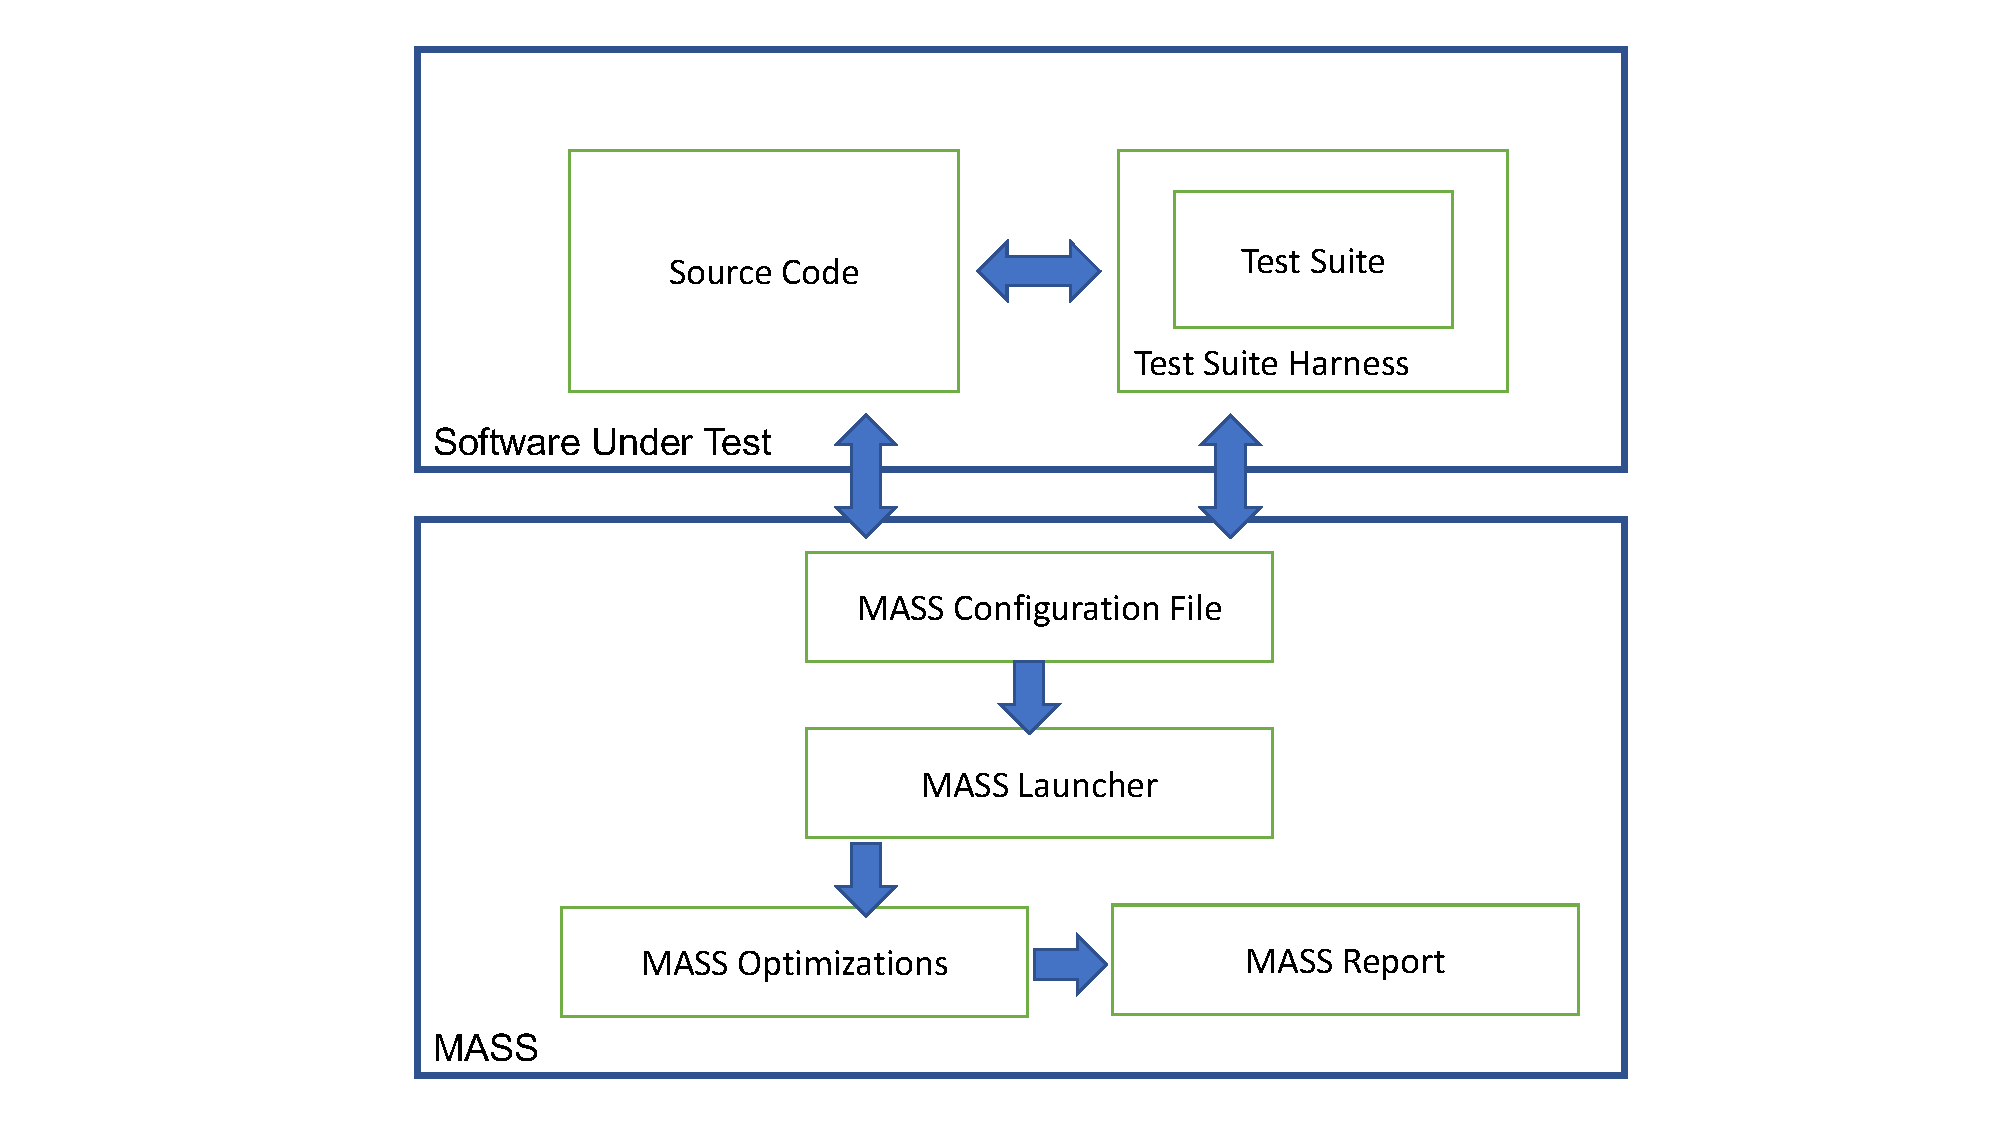
\includegraphics[width=0.7\textwidth]{images/mass-external.pdf}
      \caption{System block diagram of MASS' external interfaces.}
      \label{fig:mass:external}
\end{figure}

Figure~\ref{fig:mass:external} shows MASS' external interfaces through a system block diagram.
As shown in Figure~\ref{fig:mass:external}, MASS mainly interacts with the SUT through a configuration file, where engineers shall specify a set of Bash variables that enable MASS to correctly identify the SUT paths (e.g., source code folder, test suite folder), SUT compilation commands, the SUT test suite execution commands, and the configuration of MASS itself (e.g., trivial compiler optimizations flags, mutant selection strategy, sampling rate).


% \subsection{Assumption and dependencies}

\section{SEMuS}

\subsection{Product perspective}

In this section, we provide a brief description of the external interfaces of the Symbolic Execution-based Mutation Analysis Engine for Space Software (SEMuS).

SEMuS is an extension of SEMu, a symbolic execution engine based on KLEE, for this reason the product interacts mainly with the interfaces of KLEE-SEMu, and shall be properly configured for it. Additionally, the software interacts with the SUT, since it needs to parse the source code for test template generation, and also interacts with MASS, since the software needs to process the list of mutants for which inputs shall be generated.


\subsection{Operational environment}

\begin{figure}[t]
  \centering
  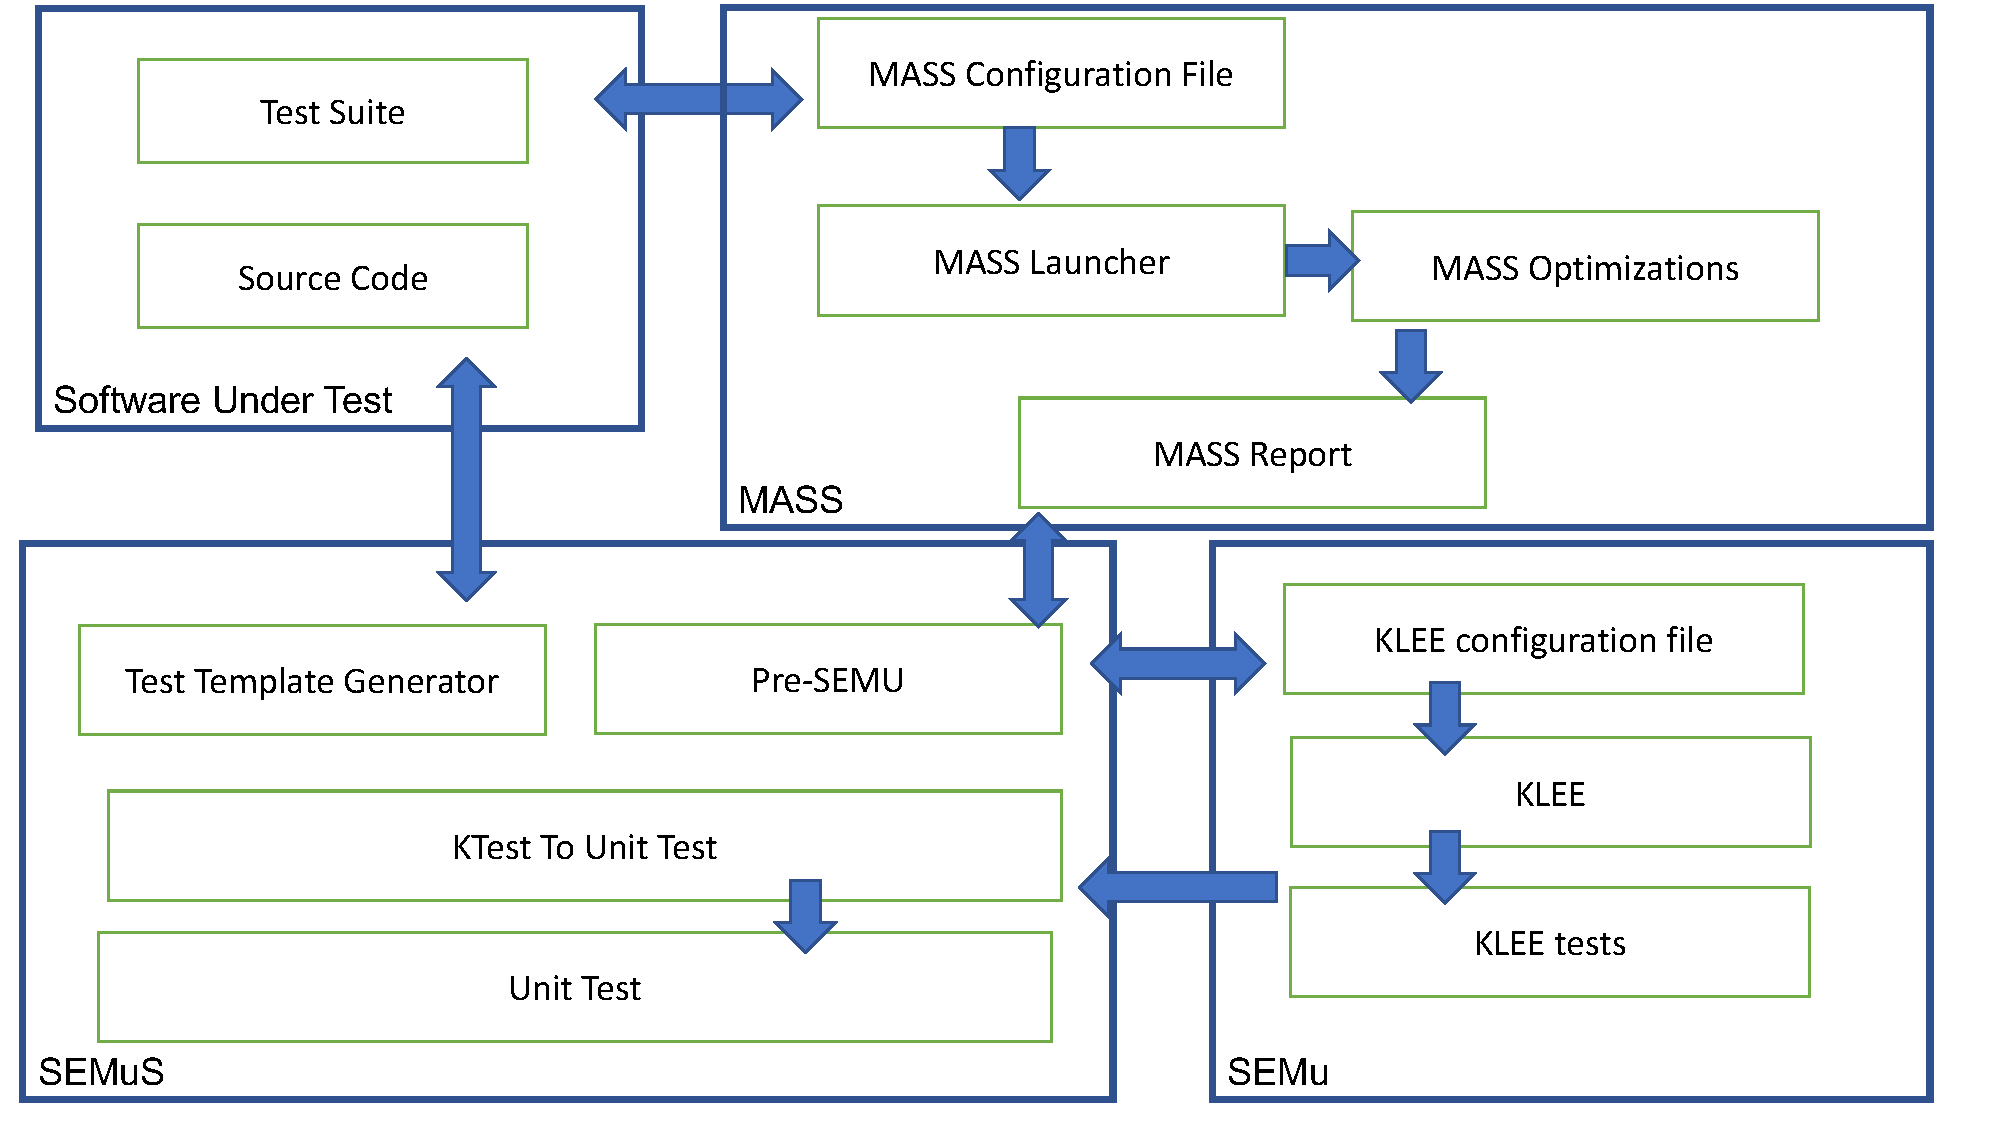
\includegraphics[width=0.7\textwidth]{images/semus-external.pdf}
      \caption{System block diagram of SEMuS' external interfaces.}
      \label{fig:semus:external}
\end{figure}

Figure~\ref{fig:semus:external} shows SEMuS' external interfaces through a system block diagram.
As shown in Figure~\ref{fig:semus:external}, SEMuS interacts with three external systems (1) the SUT, (2) the MASS toolset, and (3) the SEMu.

Firstly, SEMuS interacts with the SUT by means of a configuration file, where engineers shall specify a set of Bash variables that enable SEMuS to correctly identify the SUT paths (e.g., source code folder), SUT compilation commands, the configuration of SEMuS (e.g., output folder), and the configuration of SEMu (e.g., configuration of the heuristics, timeouts, maximum memory to be used).

Secondly, SEMuS interacts with MASS by means of the previously generated \emph{MASS report}, which provides information about the live and killed mutants. The information of live mutants is then used by SEMuS in order to generate test inputs only for the selected mutants. 
The engineers shall setup the SEMuS configuration file to provide the path to the MASS report.

Lastly, SEMuS interacts with SEMu by means of the \emph{SEMu Wrapper}, a Python script that setups the KLEE configuration file and invokes SEMu. If test inputs are generated for the specified mutants, KLEE-SEMu will produce KLEE tests that shall be processed by the \emph{KTest To Unit Test} component.



% \subsection{Assumption and dependencies}

% !TEX root = MAIN.tex

\chapter{External View of the Software}

The \FAQAS is delivered as a compressed archive consisting of source files and an installer.
The following bulletpoints provide a description of the archive's structure once uncompressed:

\begin{itemize}
	\item \texttt{FAQASFramework/}
	\begin{itemize}
		\item \texttt{SRCMutation/}: contains the source files of the component that performs code-driven mutations.
		\item \texttt{llvm-build.sh}: build script that compiles the SRCMutation component
		\item \texttt{PythonWrappers/}: contains Python script wrappers that facilitate code-driven mutations.
		\item \texttt{MASS/}: contains all the executable files and scripts that implement the methodology for code-driven mutation testing supported by  the FAQAS-Framework. They are listed below.
		\begin{itemize}
			\item \texttt{FAQAS-Setup}: contains the Bash scripts necessary to install the FAQAS-Framework.
			\item \texttt{FAQAS-GenerateCodeCoverageMatrixes}: contains the Bash scripts providing procedures to collect code coverage from the SUT.
			\item \texttt{FAQAS-GenerateMutants}: contains a Bash script that invokes the \texttt{SRCMutation} component to generate mutants.
			\item \texttt{FAQAS-CompileOptimizedMutants}: contains the scripts (in Python and Bash)  that provide the procedures to compile mutants and filter equivalent and redundant mutants based on trivial compiler optimizations.
			\item \texttt{FAQAS-CompileAndExecuteMutants}
			\begin{itemize}
				\item \texttt{FAQAS-GeneratePrioritizedTestSuite}: contains the Python and Bash scripts that provide the procedures to generate prioritized and reduced test suites from the SUT.

				\item \texttt{FAQAS-CompileAndExecute}: contains the Python and Bash scripts that provide the procedures to compile and execute the mutants against the SUT test suite. It also provides the procedures to determine the mutation stopping criterion (i.e., mutant sampling).

				\item \texttt{FAQAS-IdentifyEquivalentAndRedundantMutants}: contains the Python and Bash scripts that provides the procedures to identify equivalent mutants based on code coverage.
			\end{itemize}
			\item \texttt{FAQAS-MutationScore}: contains the Python and Bash scripts that provide the procedures to compute the mutation score and provide summarized information about the code-driven mutation testing process.
		\end{itemize}
	\end{itemize}
\end{itemize}


% !TEX root = MAIN.tex

\chapter{MASS - Operations Environment}
\label{chapter:operations}

%\REVISION{P-1}{
\section{Hardware Configuration - Single Machine}

The \MASS toolset uses a host computer with the Linux operating system. \MASS needs the following hardware requirements to be executed on single machines:

\begin{itemize}
	\item x86\_64 PC architecture
	\item 4\,096 MB of RAM
	\item Intel i3 (or equivalent) processor
\end{itemize}

\section{Hardware Configuration - High Performance Computing (HPC)}

The \MASS toolset can be also executed on High Performance Computing (HPC) infrastructures. \REVOCT{P-3}{An HPC infrastructure is a supercomputer where the computing resources of several single computer nodes are combined to achieve a high level of performance thanks to parallel execution and distribution of tasks. For replicability, in the following, we describe the main characteristics of the HPC of the University of Luxembourg, where MASS experiments had been performed.} 

\begin{itemize}
	\item HPC CPU processors: Intel Xeon E5-2680 v4 (2.4 GHz)
	\item HPC nodes memory: 112 gb
	\item Operative system: CentOS 7 x86\_64 GNU/Linux
	\item Job scheduler: \texttt{slurm 20.11.7}
\end{itemize}

Instead, these are the minimum hardware configurations to be set on HPCs for a single job:

\begin{itemize}
	\item CPU per task: 2
	\item Memory per CPU: 4\,096 MB of RAM
\end{itemize}

\section{Software Configuration}

\MASS integrates the \texttt{SRCMutation} component from \texttt{SRCIRor} mutation analysis tool\footnote{https://github.com/TestingResearchIllinois/srciror}. The installation of \texttt{SRCMutation} makes part of \MASS installation (see \ref{sec:install}).

In order to perform its tasks, \MASS also requires a few external components listed in the following:

\begin{itemize}
	\item clang-3.8
	\item r-base (package binom)
	\item jq
	\item Python-3.7 or higher (packages numpy and scipy)
	\item bash 4.4 or higher
\end{itemize}
%}

\REVOCT{P-4}{Note that these components shall be installed by the user before the actual MASS installation.}


\chapter{SEMUS - Operations Environment}
\label{chapter:semus:operationsEnv}

\section{Hardware Configuration - Single Machine}
\label{sec:semus:config:hw}

The \SEMUS toolset uses a host computer with the Linux operating system. \SEMUS needs the following hardware requirements to be executed on single machines:

\begin{itemize}
	\item x86\_64 PC architecture
	\item 4\,096 MB of RAM
	\item Intel i3 (or equivalent) processor
\end{itemize}

\REVFR{A6}{Execution with HPC is feasible, however, given that test generation is fast it can be achieved also with a single machine. Also, even in case of relying on an HPC, it is first necessary to generate test templates, which requires manual intervention and thus it is easier to be performed with a standard development environment (i.e., a single machine).
}

\section{Software Configuration}

\SEMUS integrates \SEMU, a symbolic execution-based mutation analysis engine, and thus it is necessary to install it before running \SEMUS. \SEMUS includes a Dockerfile that provides the necessary commands to install \SEMU and \SEMUS.

In order to perform its tasks, \SEMUS requires these components previously installed:

\begin{itemize}
	\item \texttt{Docker} (\texttt{docker-ce} \texttt{docker-ce-cli} \texttt{containerd.io})
\end{itemize}


\chapter{DAMAt - Operations Environment}
\label{chapter:dama:operationsEnv}

\section{Hardware Configuration - Single Machine}

The \DAMA toolset uses a host computer with the Linux operating system. \DAMA needs the following hardware requirements to be executed on single machines:

\begin{itemize}
	\item x86\_64 PC architecture
	\item 4\,096 MB of RAM
	\item Intel i3 (or equivalent) processor
\end{itemize}

% \section{Hardware Configuration - HPC}
%
% The \DAMA toolset can be also executed on HPC infrastructures. These are the minimum hardware configurations to be set on HPCs for a single job:
%
% \begin{itemize}
% 	\item CPU per task: 2
% 	\item Memory per CPU: 4\,096 MB of RAM
% \end{itemize}

\section{Software Configuration}

In order to perform its tasks, \DAMA also requires a few external components listed in the following:

\begin{itemize}
	\item \texttt{Python 3.6.8} or higher
	\item \texttt{GNU bash, version 4.2.46} or higher
\end{itemize}


% !TEX root = MAIN.tex

\chapter{MASS - Operations Manual}

\section{Set-up and Initialization}
\label{sec:install}

\MASS depends on LLVM for source code mutation. For this reason, a full LLVM-3.8.1 installation is necessary preceding the installation of the \texttt{SRCMutation} component. For this procedure, a Bash script is provided.

The following shell command installs the corresponding dependencies and the \texttt{SRCMutation} component.

\begin{lstlisting}[language=bash]
  $ ./llvm-build.sh
\end{lstlisting}

\subsection{Dependencies}

%\TODO{should we add the LLVM version?}
%\OSCAR{llvm is installed automatically in the previous step, only clang3.8 is necessary}

\begin{itemize}
	\item Linux packages: \texttt{clang 3.8}, \texttt{r-base}, \texttt{jq}, \texttt{Python 3.7} or higher
	\item R packages: \texttt{binom}
	\item Python packages: \texttt{numpy}, \texttt{scipy}
\end{itemize}


\section{Getting started}

\subsection{Initialization of the MASS workspace}

% \DONE{I think "shall" should be simply removed, "\MASS creates" "are stored".}

\MASS creates a workspace folder where all the steps from the methodology are stored.

An installation Bash script is provided for the creation of this workspace, the script can be found on \texttt{\$FAQAS/MASS/FAQAS-Setup/install.sh}

To use the installation script the shell variable \texttt{INSTALL\_DIR} has to be set:

\begin{lstlisting}[language=bash]
  $ export INSTALL_DIR=/opt/DIRECTORY
\end{lstlisting}

%\DONE{the meaning of the ollowing is not clear. Add an example.}
If the \texttt{INSTALL\_DIR} directory must be binded inside a container. In addition, also the shell variable \texttt{EXECUTION\_DIR} has to be set. This step is optional.

For instance, \MASS has been installed on \texttt{/opt/MASS\_WORKSPACE} (i.e., the \texttt{INSTALL\_DIR}), and \MASS will be executed inside a container, but on a different directory such as \\\texttt{/home/user/MASS\_WORKSPACE} (i.e., the \texttt{EXECUTION\_DIR}). The use of both environment variables enable this differentiation.


After setting the corresponding environment variables, the following commands are necessary to create the \MASS workspace folder:

\begin{lstlisting}[language=bash]
  $ cd $FAQAS/MASS/FAQAS-Setup
  $ ./install.sh
\end{lstlisting}

Once the installation folder has been created, the folder shall contain the following structure and files:

\begin{itemize}
	\item \texttt{Launcher.sh}: \MASS single launcher; the script executes all the steps of the methodology in one command.
	\item \texttt{mass\_conf.sh}: \MASS configuration file; the file has to be configured before being able to execute \MASS.
	\item \texttt{mutation\_additional\_functions.sh}: Bash script that must be filled by the application engineer before executing \MASS.
	\item \texttt{MASS\_STEPS\_LAUNCHERS/}: folder containing all the single launchers for each step of the \MASS methodology.
	\begin{itemize}
		\item \texttt{MASS\_STEPS\_LAUNCHERS/PrepareSUT.sh}: launcher for the script that prepares the SUT and collects information about the SUT test suite.
		\item \texttt{MASS\_STEPS\_LAUNCHERS/GenerateMutants.sh}: launcher for the generation of mutants.
		\item \texttt{MASS\_STEPS\_LAUNCHERS/CompileOptimizedMutants.sh}: launcher for the trivial compiler optimization step.
		\item \texttt{MASS\_STEPS\_LAUNCHERS/OptimizedPostProcessing.sh}: launcher for the post-processing of the trivial compiler optimization step.
		\item \texttt{MASS\_STEPS\_LAUNCHERS/GeneratePTS.sh}: launcher for the generation of prioritized and reduced test suites.
		\item \texttt{MASS\_STEPS\_LAUNCHERS/ExecuteMutants.sh}: launcher for the execution of mutants against the SUT test suite.
		\item \texttt{MASS\_STEPS\_LAUNCHERS/IdentifyEquivalents.sh}: launcher for the identification of equivalent mutants based on code coverage.
		\item \texttt{MASS\_STEPS\_LAUNCHERS/MutationScore.sh}: launcher for the computation of the mutation score and final reporting.
		\item \texttt{MASS\_STEPS\_LAUNCHERS/PrepareMutants\_HPC.sh}: HPC launcher that prepares the mutants workspace for the execution on HPCs.
		\item \texttt{MASS\_STEPS\_LAUNCHERS/ExecuteMutants\_HPC.sh}: HPC launcher that executes mutants on HPCs.
		\item \texttt{MASS\_STEPS\_LAUNCHERS/PostMutation\_HPC.sh}: HPC launcher that assesses past mutant executions, and decides whether more mutant executions are needed.
	\end{itemize}

\end{itemize}

\subsection{MASS Configuration}

There are three Bash scripts that should be edited by the engineer to configure \MASS. These three scripts enable \MASS to correctly identify the SUT paths (e.g., source code folder, test suite folder), the SUT compilation commands, the SUT test suite execution commands, and the configuration of \MASS itself (e.g., trivial compiler optimizations flags, mutant selection strategy, sampling rate).

%\DONE{We should have a table with the script name, the parameter to be configured and a description}
Table~\ref{table:to_configure} provides a summary of \MASS configuration files, their parameters, and a brief description. A detailed description of the MASS configuration files follows.


% !TEX root =  ../MAIN.tex

\begin{table}[tb]
\footnotesize
\centering
\caption{\MASS minimal set of parameters to be configured.}
\label{table:to_configure}
\begin{tabular}{llp{7.5cm}}
\hline
\textbf{Script Name}  & \textbf{Parameter} &  \textbf{Description} \\
\hline
mass\_conf.sh & BUILD\_SYSTEM &  Specifies the building system type.\\
& PROJ &  Path of the SUT root  directory.\\
& PROJ\_SRC &  Path of the SUT source directory.\\
& PROJ\_TST &  Path of the SUT test  directory.\\
& PROJ\_COV &  Path of the directory with SUT coverage information.\\
& PROJ\_BUILD &  Path of the directory where the compiled binary is stored.\\
& ORIGINAL\_MAKEFILE &  Path to the original build script.\\
& COMPILATION\_CMD &  Compilation command of the SUT.\\
\hline
PrepareSUT.sh & None &  Commands shall be provided manually.\\
\hline
mutation\_additional\_functions.sh & run\_tst\_case  &  Implementation of the Bash function run\_tst\_case that executes the test case passed as a parameter.\\
\hline
\end{tabular}
\end{table}



%The last intervention, regards providing a template of the original build script for the trivial compiler optimizations step. More details are provided in the following.



\subsubsection{Edit mass\_conf.sh}

Within file \texttt{\$INSTALL\_DIR/mass\_conf.sh} there are multiple environment variables that must be set; they are shown in Listing~\ref{listing:MASS:conf}.

%\DONE{You should always refer to Figures/Listings in appropriate manner. However, this "style" is ok for the running example.}

\begin{lstlisting}[language=bash,label=listing:MASS:conf,caption=Excerpt of mass\_conf.sh file.]
	# set SRCIROR path
	export SRCIROR=

	# set workspace directory path where MASS files can be stored (i.e., $INSTALL_DIR)
	export APP_RUN_DIR=

	# specifies the building system, available options are "Makefile" and "waf"
	export BUILD_SYSTEM=

	# directory root path of the SUT
	export PROJ=

	# directory source path of the SUT
	export PROJ_SRC=

	# directory test path of the SUT
	export PROJ_TST=

	# directory coverage path of the SUT
	export PROJ_COV=

	# directory path where the compiled binary is stored
	export PROJ_BUILD=

	# list of folders not to be included during coverage analysis, name folders shall be separated by '\|'
	export COVERAGE_NOT_INCLUDE=

	# filename of the compiled file or library
	export COMPILED=

	# path to the original build script
	export ORIGINAL_MAKEFILE=

	# compilation command of the SUT, the command shall be specified as a Bash array, e.g., (). Special characters shall be escaped.
	export COMPILATION_CMD=

	# additional commands for compiling the SUT (e.g., setup of workspace), the command shall be specified as a Bash array, e.g., (). Special characters shall be escaped.
	export ADDITIONAL_CMD=

	# command to be executed after each test case execution (optional), the command shall be specified as a Bash array, e.g., (). Special characters shall be escaped.
	export ADDITIONAL_CMD_AFTER=

	# compilation command for TCE analysis, the command shall be specified as a Bash array, e.g., (). Special characters shall be escaped.
	export TCE_COMPILE_CMD=

	# command to clean installation of the SUT, the command shall be specified as a Bash array, e.g., (). Special characters shall be escaped.
	export CLEAN_CMD=

	# relative path to location of gcov files (i.e., gcda and gcno files)
	export GC_FILES_RELATIVE_PATH=
\end{lstlisting}

Furthermore, the following specific \MASS variables must be set (See Listing~\ref{listing:MASS:conf_2}):

\begin{lstlisting}[language=bash, label=listing:MASS:conf_2, caption=\MASS specific variables. Excerpt of mass\_conf.sh file.]
	# specify if MASS will be executed on an HPC, possible values are "true" or "false"
	export HPC=

	# TCE flags to be tested, the flags shall be specified as a Bash array, e.g., ("-O0" "-O1").
	export FLAGS=

	# set if MASS should be executed with a prioritized and reduced test suite, possible values are "true" or "false"
	export PRIORITIZED=

	# set sampling technique, possible values are "uniform", "stratified", and "fsci"
	# note: if "uniform" or "stratified" is set, $PRIORITIZED must be "false"
	export SAMPLING=

	# set sampling rate if whether "uniform" or "stratified" sampling has been selected
	export RATE=
\end{lstlisting}

\subsubsection{Edit PrepareSUT.sh}

% \TODO{The title should be changed, probably it should become something like \emph{Edit PrepareSUT.sh}. My main problem is that I cannot map this section to something describe before, it comes out of the blue. Also, shouldn't it be a subsubsection? I would expect to have in 4.2.2 the list of all the files to be editng and in the following subsubsections a description for each of them.}

To configure \MASS to work with the SUT, the engineer should also edit the Bash file \\\begin{small}\texttt{\$INSTALL\_DIR/MASS\_STEPS\_LAUNCHER/PrepareSUT.sh}\end{small}. The following actions shall be performed by the engineer:

\begin{enumerate}
	\item Provide commands to generate a compilation database file \texttt{compile\_commands.json} of the SUT. Note that the paths defined within the database file must be full paths. The compilation database file provides the necessary compilation commands of each source for the source mutation step of the methodology.
%	\DONE{Not clear why the engineer should do what written above}
%	\TODO{STill not clear}
	\item Provide commands to compile the SUT;
	\item Provide additional commands to prepare the SUT workspace (optional);
	\item Provide commands to execute the SUT test suite iteratively over each test case; more precisely, the engineer should do the following:
	\begin{itemize}
		\item After the command executing a a test case add a call to \\\texttt{\$MASS/FAQAS-GenerateCodeCoverageMatrixes/FAQAS-CollectCodeCoverage.sh} script;
		\item the script \texttt{FAQAS-CollectCodeCoverage.sh} shall be invoked with two arguments: (i) the test case name, and (ii) the time taken to run the test case in seconds.
	\end{itemize}
\end{enumerate}

\subsubsection{Mutation Script Configuration}

The mutation script configuration file is the Bash file \texttt{mutation\_additional\_functions.sh}. In it, the engineer is expected to implement the Bash function \texttt{run\_tst\_case}.
%Fabrizio: not clear what you mena below
%; must be implemented by the engineer to guarantee a correct mutation testing process.
This function shall receive as argument the name of the test case to be executed. It should execute the command for running the specified test case.
%Why "Particularly" ?
%Particularly,
The function shall return 0, if the test case passes; it shall return 1 if the test case fails.


\subsubsection{Build Script for Compiler Optimizations}

The SUT engineer shall provide a build script for the SUT. Such script shall be placed in the same folder where the original build script resides (a different name shall be used). The script shall have the following characteristics:

\begin{itemize}
	\item The script shall not contain any debugging flag within compilation/linking commands;
	\item The script shall not contain any code coverage flag within compilation/linking commands;
	\item The script shall contain a placeholder for the compiler optimization option, specifically the placeholder \texttt{TCE};
	\item The script shall contain a 'sort' command in the list of source files to be compiled, to ensure that source files are always compiled in the same order;
	%\DONE{Not clear what a source dependency list is, example?}

	In the case of a Makefile, it can be achieved with the following command:

	\texttt{SRC=\$(sort \$(wildcard \$(SourceFolder/*.c))}

	\item The script shall be named the same as the original build script, but with an ending '.template'.
\end{itemize}


\subsection{Running MASS on Single Machines}
\label{sec:singlelaunch}

%\DONE{Add a paragraph that explains that you are going to describe two ways of running MASS}

\MASS can be executed in two modes, \emph{single machine} and \emph{shared resources mode}. The single machine mode provides the advantage of running \MASS in an unsupervised mode, executing the methodology on one step. Instead, the shared resources facilities mode gives the possibility of running multiple steps in parallel and executing a higher number of mutants, in a similar time frame, with respect to the single machine mode. In this section we describe the \emph{single machine}, Section \ref{sec:shared} covers the \emph{shared resources mode}.

%\TODO{You should either (a) specify the files generated for each step, or (b) put a sentence saying that the output/inputs of each step are described in the specification document XY (and you have t draft it by reciclying the old SSS.}
%
%The inputs and outputs of each step are described in the specification document XY.


\subsubsection{One Step Launcher}

The single machine mode gives the possibility of running \MASS in one step, by executing all the eight steps of the framework with one command. The one step launcher will execute the following steps sequentially:

\begin{enumerate}
	\item PrepareSUT
	\item GenerateMutants
	\item CompileOptimizedMutants
	\item OptimizedPostProcessing
	\item GeneratePTS
	\item ExecuteMutants
	\item IdentifyEquivalents
	\item MutationScore
\end{enumerate}

To execute the one step launcher, the following command shall be provided:

\begin{lstlisting}[language=bash]
  $ ./Launcher.sh
\end{lstlisting}

\subsubsection{Multiple Step Launchers}
\label{sec:launchers}

The single machine mode also gives the possibility to run \MASS by executing all the eight steps of the framework through independent commands.
The multiple steps of the methodology and their respective commands are described in the following.

\begin{enumerate}
	\item \textbf{Prepare the SUT} step can be executed with the following command:

	\begin{lstlisting}[language=bash]
	  $ ./MASS_STEPS_LAUNCHER/PrepareSUT.sh
\end{lstlisting}

	\item \textbf{Generate Mutants} step can be executed with the following command:

	\begin{lstlisting}[language=bash]
	  $ ./MASS_STEPS_LAUNCHER/GenerateMutants.sh
\end{lstlisting}

	\item \textbf{Compile Optimized Mutants} step can be executed with the following command:

	\begin{lstlisting}[language=bash]
	  $ ./MASS_STEPS_LAUNCHER/CompileOptimizedMutants.sh
\end{lstlisting}

	\item \textbf{Compile Optimized Mutants Post-Processing} step can be executed with the following command:

	\begin{lstlisting}[language=bash]
	  $ ./MASS_STEPS_LAUNCHER/OptimizedPostProcessing.sh
\end{lstlisting}

	\item \textbf{Generate Prioritized and Reduced Test Suites} step can be executed with the following command:

	\begin{lstlisting}[language=bash]
	  $ ./MASS_STEPS_LAUNCHER/GeneratePTS.sh
\end{lstlisting}

	\item \textbf{Execute mutants} step can be executed with the following command:

	\begin{lstlisting}[language=bash]
	  $ ./MASS_STEPS_LAUNCHER/ExecuteMutants.sh
\end{lstlisting}

	\item \textbf{Identify Equivalent Mutants based on Code Coverage} step can be executed with the following command:

	\begin{lstlisting}[language=bash]
	  $ ./MASS_STEPS_LAUNCHER/IdentifyEquivalents.sh
\end{lstlisting}

	\item \textbf{Computer Mutation Score} step can be executed with the following command:

	\begin{lstlisting}[language=bash]
	  $ ./MASS_STEPS_LAUNCHER/MutationScore.sh
\end{lstlisting}
\end{enumerate}


\subsection{Running MASS on Shared Resources Facilities}
\label{sec:shared}

Given that resources from HPC infrastructures has to be requested for every performed tasks, it is not possible to run all the steps from \MASS in one step.
However, since resources can be requested accordingly, \MASS can perform multiple steps simultaneously, enhancing the capabilities of the toolset. With an HPC, for example, \MASS could analyze more mutants than if \MASS was executed on a single machine.

The multiple steps of the methodology and their respective commands are described in the following.

\begin{enumerate}
	\item \textbf{Prepare the SUT} step can be executed with the following command:

	\begin{lstlisting}[language=bash]
	  $ ./MASS_STEPS_LAUNCHER/PrepareSUT.sh
\end{lstlisting}

	\item \textbf{Generate Mutants} step can be executed with the following command:

	\begin{lstlisting}[language=bash]
	  $ ./MASS_STEPS_LAUNCHER/GenerateMutants.sh
\end{lstlisting}

	\item \textbf{Compile Optimized Mutants}: 
	%If the environment variable \texttt{HPC} is set to \texttt{true}. 
	A parameter shall be passed to the launcher script to indicate the chosen optimization level. If six levels of optimizations are defined, then numbers between zero and five can be provided.

	\begin{lstlisting}[language=bash]
	  $ level=0
	  $ ./MASS_STEPS_LAUNCHER/CompileOptimizedMutants.sh $level
\end{lstlisting}

	\item \textbf{Compile Optimized Mutants Post-Processing} step can be executed with the following command:

	\begin{lstlisting}[language=bash]
	  $ ./MASS_STEPS_LAUNCHER/OptimizedPostProcessing.sh
\end{lstlisting}

	\item \textbf{Generate Prioritized and Reduced Test Suites} step can be executed with the following command:

	\begin{lstlisting}[language=bash]
	  $ ./MASS_STEPS_LAUNCHER/GeneratePTS.sh
\end{lstlisting}

	\item \textbf{Prepare mutants} step can be executed with the following command:

	\begin{lstlisting}[language=bash]
	  $ ./MASS_STEPS_LAUNCHER/PrepareMutants_HPC.sh
\end{lstlisting}

	\item \textbf{Execute mutants}: The launcher script receives two parameters: the first parameter is the number of the mutant to be executed, defined as ${1..M}$, being M the total number of mutants. The total number of mutants can be derived from the folder \texttt{\$INSTALL\_DIR/hpc-src-mutants}.
	The second parameter defines if the test suite has to be executed in a reduced fashion or not. The possible values are ``true'' and ``false''.

	\begin{lstlisting}[language=bash]
	  $ nr_mutant=1
	  $ reduced="false"
	  $ ./MASS_STEPS_LAUNCHER/ExecuteMutants_HPC.sh $nr_mutant $reduced
\end{lstlisting}

	\item \textbf{Post-mutation execution}: The launcher script receives two numbers as parameters, a minimum and a maximum value, that represent the range of mutants to assess. The assessment consists of evaluating if more mutant executions are needed.

	\begin{lstlisting}[language=bash]
	  $ min=1
	  $	max=700
	  $ ./MASS_STEPS_LAUNCHER/PostMutation_HPC.sh $min $max
\end{lstlisting}

	\item \textbf{Identify Equivalent Mutants based on Code Coverage} step can be executed with the following command:

	\begin{lstlisting}[language=bash]
	  $ ./MASS_STEPS_LAUNCHER/IdentifyEquivalents.sh
\end{lstlisting}

	\item \textbf{Computer Mutation Score} step can be executed with the following command:

	\begin{lstlisting}[language=bash]
	  $ ./MASS_STEPS_LAUNCHER/MutationScore.sh
\end{lstlisting}
\end{enumerate}

\subsection{MASS results}

After the execution of \MASS the results are stored in dedicated folders. Such folders are defined as follows:

\begin{enumerate}
	\item Prepare SUT: the results of this step are stored in the folder \texttt{COV\_FILES}. Besides the coverage files, it contains (i) the coverage matrices, and (ii) the timeout file.
	\item Generate Mutants: the results of this step are stored in the folder \texttt{src-mutants}, it contains all mutant sources.
	\item Compile Optimized Mutants: the results of this step are stored in the folder \texttt{COMPILED} that contains one folder for each optimisation level.
	\item Compile Optimized Mutants Post-Processing: the results of this step are stored in the folder \texttt{COMPILED}. Specifically, it generates four lists: (i) list of all mutants, (ii) list of nonequivalent and nonredundant mutants, (iii) list of equivalent mutants, and (iv) list of redundant mutants.
	\item Generate Prioritized and Reduced Test Suites: the results of this step are stored in the folder \texttt{PRIORITIZED}, which contains one file with the prioritized and reduced test suites, and one file with the prioritized test suites.
	\item Execute Mutants: the results of this step are stored in the folder \texttt{MUTATION}. This step produces several files and folders:
	\begin{itemize}
		\item \texttt{main.csv}: complete mutation traces
		\item \texttt{sampled\_mutants}: list of sampled mutants to be executed
		\item \texttt{all\_live}: list of live mutants
		\item \texttt{all\_killed}: list of killed mutants
		\item \texttt{traces\_live}: live mutants traces
		\item \texttt{traces\_killed}: killed mutants traces
		\item \texttt{mutant folder}: there is one folder for each executed mutant, this folder contains the mutant code coverage information and test cases execution logs.
	\end{itemize}
	\item Identify Equivalent Mutants based on Code Coverage: the results of this step are stored in the folder \texttt{DETECTION}.
	\item Compute Mutation Score: the results of this step are stored in folder \texttt{RESULTS}. Particularly, the file \texttt{MASS\_RESULTS} contains the final output of \MASS.
\end{enumerate}


% \section{Mode selection and control}

% \section{Normal Operations}

\section{Normal Termination}

%\DONE{"The SUM shall describe how the user can cease or interrupt use of the software and how to determine whether normal termination or cessation has occurred."}

Each methodology step of \MASS is executed when invoked and computes a result. There is no software interruption foreseen during the computation and the procedure terminates by returning the result.
If the engineer decides to interrupt \MASS execution, it can be done by sending a signal interrupt \texttt{SIGINT} to the running process.

\section{Error Conditions}

%\DONE{Can 't we say anything about each program not returning any error message?}

There is no error condition handling in the \FAQAS. If all preconditions are met, there should not be any error.

\section{Recover Runs}

%\DONE{Shall we say that an engineer can restart the process form a task if all the precondiions are met?}

If for any reason the execution of \MASS is interrupted, an engineer can restart the process from a specific task if all preconditions are met. This is possible since each \MASS step work by processing data that is permanently stored by previous steps.


\STARTCHANGEDWPT
% !TEX root = MAIN.tex

\chapter{SEMUS - Operations Manual}
\label{chapter:semus:operations}

\section{Set-up and Initialization}
\label{sec:install:semus}

\SEMUS depends directly on \SEMU for test inputs generation, and \MASS for mutant generation.

For this reason, we provide a Dockerfile containing all the commands necessary to download, install and prepare a full installation of \SEMU and MASS. The Dockerfile can be found at \texttt{\SEMUS/Dockerfile}. The installation will take place the first time the Docker image is created through the Bash script \texttt{cd\_semu\_docker.sh}, no further installation is required for now.

\subsection{Dependencies}

%\TODO{should we add the LLVM version?}
%\OSCAR{llvm is installed automatically in the previous step, only clang3.8 is necessary}

\begin{itemize}
	\item Linux packages: \texttt{docker-ce} \texttt{docker-ce-cli} \texttt{containerd.io}
\end{itemize}


\section{Getting started}

\subsection{Initialization of the \SEMUS workspace}
\label{sec:semus:initialization}

\SEMUS needs a dedicated folder structure for running the test generation on a case study. 
For this reason, the engineer shall create the following directory structure under the folder \texttt{case\_studies}, assuming the name of the case study is stored in the variable \texttt{\$SUT}:

\begin{itemize}
	\item \texttt{case\_studies/\$SUT/:}
	\begin{itemize}
		\item \texttt{scripts/}
		\item \texttt{util\_codes/}
		\item \texttt{WORKSPACE/}
	\end{itemize}
\end{itemize}

After the creation of the folder structure, the engineer shall copy the scripts for (1) creating the mutants, (2) running the toolset, (3) configuring \SEMUS. The commands for copying these files are provided below:

\begin{lstlisting}[language=bash]
  $ cd case_studies/MLFS/scripts
  $ cp create_mutants.sh run.sh docker_run.sh faqas_semus_config.sh ../../$SUT/scripts
\end{lstlisting}

At this step, the engineer shall also provide a compilation database file of the SUT, to be placed inside \texttt{\$SUT/scripts} with the name \texttt{compile\_commands.json}. Note that the paths defined within the database file must be full paths. The compilation database file provides the necessary compilation commands of each source for the source mutation and the test generation steps of the methodology.

Next, the engineer shall copy the script necessary for generating the test templates for guiding the test generation. This can be done through the following commands:

\begin{lstlisting}[language=bash]
  $ cd case_studies/MLFS/util_codes
  $ cp call_generate_direct.sh ../../$SUT/util_codes
\end{lstlisting}

Last, the engineer shall place inside the folder \texttt{case\_studies/\$SUT/WORKSPACE/DOWNLOADED} (1) the SUT source code, and (2) the list of live mutants (provided by \MASS output).

\subsection{\SEMUS Configuration}

There is one Bash script that should be edited by the engineer to configure \SEMUS. The script enable \SEMUS to correctly identify the SUT paths (e.g., source code folder), the SUT compilation commands, output folder, and the configuration of \SEMUS itself (e.g., configuration of the heuristics, maximum memory, test generation timeout).

% !TEX root =  ../MAIN.tex

\begin{table}[t]
\tiny
\centering
\caption{SEMuS parameters to be configured.}
\label{table:to_conf_semus}
\begin{tabular}{lp{8.5cm}}
\hline
\textbf{Parameter}  &  \textbf{Description} \\
\hline
FAQAS\_SEMU\_CASE\_STUDY\_TOPDIR &  Root folder of the case study \\
FAQAS\_SEMU\_CASE\_STUDY\_WORKSPACE &  SEMuS workspace for the case study \\
FAQAS\_SEMU\_OUTPUT\_TOPDIR & SEMuS output folder, to be placed inside the workspace \\
FAQAS\_SEMU\_GENERATED\_MUTANTS\_TOPDIR & Root folder for storing the generated mutants \\
FAQAS\_SEMU\_REPO\_ROOTDIR &  Root folder of the case study source code\\
FAQAS\_SEMU\_ORIGINAL\_SOURCE\_FILE & Path of the source file under analysis \\
FAQAS\_SEMU\_COMPILE\_COMMAND\_SPECIFIED\_SOURCE\_FILE & Name of the source file under analysis \\
FAQAS\_SEMU\_GENERATED\_MUTANTS\_DIR & Folder for storing the generated mutants for the specified source file\\
FAQAS\_SEMU\_BUILD\_CODE\_FUNC\_STR & Bash function for building the source file under analysis, to be specified in string format\\
FAQAS\_SEMU\_BUILD\_LLVM\_BC & Bash function for building the source file to LLVM bitcode \\
FAQAS\_SEMU\_META\_MU\_TOPDIR &  Root folder for the meta mutant \\
FAQAS\_SEMU\_GENERATED\_META\_MU\_SRC\_FILE &  Path of the source file (i.e., C file) of the meta mutant \\
FAQAS\_SEMU\_GENERATED\_META\_MU\_BC\_FILE &  Path of the source file (i.e., LLVM bitcode file) of the meta mutant \\
FAQAS\_SEMU\_GENERATED\_META\_MU\_MAKE\_SYM\_TOP\_DIR &  Folder for storing intermediate files for the generated inputs \\
FAQAS\_SEMU\_GENERATED\_TESTS\_TOPDIR &  Folder for storing the generated inputs \\
FAQAS\_SEMU\_TEST\_GEN\_TIMEOUT & Timeout in seconds for the test generation process \\
FAQAS\_SEMU\_HEURISTICS\_CONFIG & Configuration array for SEMu heuristics \\
FAQAS\_SEMU\_TEST\_GEN\_MAX\_MEMORY & Maximum test generation memory in MB \\
FAQAS\_SEMU\_STOP\_TG\_ON\_MEMORY\_LIMIT & Parameter to stop test generation when the memory limit is reached \\
FAQAS\_SEMU\_TG\_MAX\_MEMORY\_INHIBIT & Parameter to stop forking states when the memory limit is reached \\
\hline
\end{tabular}
\end{table}




Table~\ref{table:to_conf_semus} provides a summary of \SEMUS configuration files and a brief description. A detailed description of the SEMuS configuration file follows.


\subsubsection{Edit faqas\_semus\_config.sh}

Within file \texttt{faqas\_semus\_config.sh} there are multiple environment variables that must be set; they are shown in Listing~\ref{listing:SEMUS:conf}.

\begin{lstlisting}[language=bash,label=listing:SEMUS:conf,caption=faqas\_semus\_conf.sh file.]

# Root folder of the case study
FAQAS_SEMU_CASE_STUDY_TOPDIR=

# SEMuS workspace for the case study
FAQAS_SEMU_CASE_STUDY_WORKSPACE=$

# SEMuS output folder, to be placed inside the workspace
FAQAS_SEMU_OUTPUT_TOPDIR=

# Root folder for storing the generated mutants
FAQAS_SEMU_GENERATED_MUTANTS_TOPDIR=

# Root folder of the case study source code
FAQAS_SEMU_REPO_ROOTDIR=

# Full path of the source file under analysis
FAQAS_SEMU_ORIGINAL_SOURCE_FILE=

# Relative path of the source file under analysis
FAQAS_SEMU_COMPILE_COMMAND_SPECIFIED_SOURCE_FILE=

# Folder for storing the generated mutants for the specified source file
FAQAS_SEMU_GENERATED_MUTANTS_DIR=

# Bash function for building the source file under analysis, to be specified in string format
FAQAS_SEMU_BUILD_CODE_FUNC_STR='FAQAS_SEMU_BUILD_CODE_FUNC() { }'

# Bash function for building the source file to LLVM bitcode
FAQAS_SEMU_BUILD_LLVM_BC() { }

# Root folder for the meta mutant
FAQAS_SEMU_META_MU_TOPDIR=$FAQAS_SEMU_OUTPUT_TOPDIR/meta_mu_topdir

# Path of the source file (i.e., C file) of the meta mutant
FAQAS_SEMU_GENERATED_META_MU_SRC_FILE=

# Path of the source file (i.e., LLVM bitcode file) of the meta mutant
FAQAS_SEMU_GENERATED_META_MU_BC_FILE=

# Folder for storing intermediate files for the generated inputs 
FAQAS_SEMU_GENERATED_META_MU_MAKE_SYM_TOP_DIR=

# Folder for storing the generated inputs 
FAQAS_SEMU_GENERATED_TESTS_TOPDIR=

# Timeout in seconds for the test generation process
FAQAS_SEMU_TEST_GEN_TIMEOUT=

# Configuration array for SEMu heuristics. The accepted values of 'PSS' are 'RND' for random and 'MDO' for minimum distance to output
FAQAS_SEMU_HEURISTICS_CONFIG='{
        "PL": 
        "CW": 
        "MPD": 
        "PP": 
        "NTPM": 
        "PSS": 
}'

# Maximum test generation memory in MB
FAQAS_SEMU_TEST_GEN_MAX_MEMORY=

# Parameter to stop test generation when the memory limit is reached
FAQAS_SEMU_STOP_TG_ON_MEMORY_LIMIT=

# Parameter to stop forking states when the memory limit is reached
FAQAS_SEMU_TG_MAX_MEMORY_INHIBIT=

\end{lstlisting}

\TODO{Add the listing configured for MLFS or ASN and comment it with a sentence here.}

\subsection{Running \SEMUS}
\label{sec:semuslaunch}

To run \SEMUS is necessary to generate the test templates as first step; there is a dedicated Bash script for doing so:

\begin{lstlisting}[language=bash]
 $ case_studies/$SUT/util_codes/call_generated_direct.sh
\end{lstlisting}

The previous command will generate inside the directory \texttt{case\_studies/\$SUT/util\_codes} one folder for each source under analysis, and inside of these folders, one template for each function under test.

The test generation process can be started with the command shown in Listing~\ref{listing:semus_launch}. 

Note the following:
\begin{itemize}
	\item the first time the command is invoked, Docker will install all the dependencies of \SEMUS (i.e., \SEMU and \MASS).
	\item the environment variable \texttt{ENV\_FAQAS\_SEMU\_SRC\_FILE} has to be set before invoking; this variable indicates the source file for which the test generation will be targeted
\end{itemize}

\begin{lstlisting}[language={}, label=listing:semus_launch]
ENV_FAQAS_SEMU_SRC_FILE=source.c ./docker_run.sh [<starting-step>] [<mutants-list-file> <output-dir-for-pre-semu-and-semu>]
\end{lstlisting}

Where:
\begin{itemize}
	\item starting-step: is the step of the pipeline from which to start, possible values are \texttt{\{mutation, compile, presemu, semu,unittests\}}
	\begin{itemize}
		\item mutation: the process starts from the mutant generation step
		\item compile: the process starts from the mutant compilation step
		\item presemu: the process starts from the preparation of the meta mutant step (i.e., Pre-SEMu)
		\item semu: the process starts from the test generation step itself
		\item unittests: the process starts from the conversion of KLEE tests to unit tests step
	\end{itemize}
	\item mutants-list-file: is the file containing the list of mutants to use during the phases pre-semu and semu.
	\item output-dir-for-pre-semu-and-semu: directory to store the output of pre-semu and semu phases, when the mutants list is specified.
\end{itemize}

An example for launching the test generation from the mutation generation step follows:

\begin{lstlisting}[language=bash]
 $ ENV_FAQAS_SEMU_SRC_FILE=source.c scripts/docker_run.sh mutation WORKSPACE/DOWNLOADED/live_mutants WORKSPACE/OUTPUT/live_mutants_output
\end{lstlisting}

\subsection{\SEMUS results}

\SEMUS results can be found at the folder \texttt{case\_studies/\$SUT/WORKSPACE/OUTPUT}:

\begin{itemize}
	\item \texttt{mutants\_generation}: this folder contains the mutant sources generated by \MASS
	\item \texttt{live\_mutants\_output/mutants\_generation}: this folder stores the source files and the compiled objects of the meta mutant files (e.g., \texttt{*.MetaMu.c} and \texttt{*.MetaMu.bc})
	\item \texttt{live\_mutants\_output/test\_generation}: this folder contains the outputs of \SEMUS concerning the test generation step, this directory contains one folder for each test template. Furthermore, it also contains the following folders:
	\begin{itemize}
		\item \texttt{direct/TEMPLATE/FAQAS\_SEMu-out/semu}: \SEMU output (e.g., KLEE tests files, execution traces)
		\item \texttt{direct/TEMPLATE/FAQAS\_SEMu-out/produced-unittests}: Unit test cases converted from \SEMU output
	\end{itemize}

\end{itemize}



\section{Normal Termination}


Each step of \SEMUS is executed when invoked and computes a result. There is no software interruption foreseen during the computation and the procedure terminates by returning the result.
If the engineer decides to interrupt \SEMUS execution, it can be done by sending a signal interrupt \texttt{SIGINT} to the running process.

\section{Error Conditions}

There is no error condition handling in the \FAQAS. If all preconditions are met, there should not be any error.

\section{Recover Runs}

%\DONE{Shall we say that an engineer can restart the process form a task if all the precondiions are met?}

If for any reason the execution of \SEMUS is interrupted, an engineer can restart the process from a specific step if all preconditions are met. This is possible since each \SEMUS step work by processing data that is permanently stored by previous steps.

% !TEX root = MAIN.tex

\chapter{\DAMA - Operations Manual}

\section{Set-up and Initialization}

\subsection{Dependencies}

\begin{itemize}
	\item \texttt{Python 3.6.8} or higher
	\item \texttt{GNU bash, version 4.2.46} or higher
\end{itemize}

\section{Getting started}

\subsection{Initialization of the \DAMA workspace}

All the script for the \DAMA pipeline are contained in the \texttt{damat-pipeline} folder.
All \DAMA steps will take place inside this folder, which shall be placed by the engineer in a path of their choosing.

The folder shall contain the following structure and files:

\begin{itemize}
	\item \texttt{DAMAt\_configure.sh}: this script defines the necessary variables for the execution of \DAMA. They shall be set by the user.
	\item \texttt{DAMAt\_probe\_generation.sh}: this script set the variables necessary to generate the data mutation API and execute the python script \texttt{generateDataMutator.py} to generate them.
	\item \texttt{DAMAt\_mutants\_launcher.sh}: this script starts the \DAMA pipeline.
	\item \texttt{generateDataMutator.py}: this is the script that generates the \DAMA mutation API.
	\item \texttt{DDB\_TEMPLATE\_header.c} and \texttt{DDB\_TEMPLATE\_footer.c}: these are templates used to generate the \DAMA API by \texttt{generateDataMutator.py}
	\item \texttt{DAMAt\_compile.sh}: this is a stub of the script used to compile a mutant, which shall be completed by the user.
	\item \texttt{DAMAt\_run\_tests.sh}: this is a stub of the script used to run the tests, which shall be completed by the user.
	\item \texttt{data\_analysis}: a folder containing five python scripts used for the generation of the final results:
	\begin{itemize}
	  \item \texttt{beautify\_results.py}: this script renders the raw results from the execution of the tests in a more readable format.
	  \item \texttt{get\_coverage.py}: this script analizes the results of the fault model coverage.
	  \item \texttt{get\_operator\_coverage.py}: this script analizes the results of the operator coverage.
	  \item \texttt{get\_stats.py}: this script produces statistics from the mutants' execution.
		\item \texttt{get\_final\_results.py}: this script produces a summary of the execution of \DAMA.
	\end{itemize}
	\item \texttt{pipeline\_scripts}: a folder containing the four scripts that make up the \DAMA pipeline:
	\begin{itemize}
		\item \texttt{DAMAt\_obtain\_coverage.sh}: this script obtains fault model coverage data in order to execute only the tests that cover each mutant.
		\item \texttt{get\_mutant\_test\_list.py}: this script produces the list of test against which avery mutant shall be executed.
	  \item \texttt{DAMAt\_compile\_and\_run\_mutants.sh}: this scripts compile each mutant and run it against the SUT test suite.
		\item \texttt{DAMAt\_data\_analysis.sh}: this script executes all the data analysis steps at the end of the execution of the \DAMA pipeline
	\end{itemize}
	\item \texttt{fault\_model.csv}: an example of a \DAMA fault model in csv format.
 	\item \texttt{tests.csv }: an example of list of test cases and nominal times in csv format.
\end{itemize}

\subsection{Writing a list of all test cases}
\label{subsec:test_list}
The user shall provide the list of all the test cases with corresponding nominal time in csv format, using the \texttt{tests.csv } file as an example.
In the first column of the csv file there shall be an identifier for the test case. The second column shall contain the nominal execution time in ms.

\begin{lstlisting}
test_01,11002
test_02,13456
test_03,58347
\end{lstlisting}

This file will be used by the \DAMA pipeline for two purposes:
\begin{enumerate}
	\item the nominal execution time will be used to set a timeout for each test case.
	\item the whole list will be used to generate a list for each mutant containing only the test cases that cover it.
\end{enumerate}

\subsection{Setting the variables for the \DAMA pipeline}

% The user shall then modify three scripts to configure the \DAMA pipeline:
% \begin{itemize}
% 	\item \texttt{DAMAt\_configure.sh}
% 	\item \texttt{DAMAt\_compile.sh}
% 	\item \texttt{DAMAt\_run\_tests.sh}
% \end{itemize}

The user must set the following variables inside the \texttt{DAMAt\_configure.sh} script
\begin{lstlisting}[language=bash]

tests_list=$DAMAt_FOLDER/tests.csv

fault_model=$DAMAt_FOLDER/fault_model.csv

buffer_type="unsigned char"

singleton="TRUE"

padding=0

\end{lstlisting}

\texttt{test_list} shall be set to the path of the csv containing the test names and execution times.
\texttt{fault_model} shall be set to the path of the csv containing the fault model of the SUT that the user shall define for the SUT.
\texttt{buffer_type} shall contain the type of the elements of the buffer that will be targeted by the mutation.
\texttt{singleton} shall be set to \texttt{TRUE} or \texttt{FALSE}. If set to \texttt{TRUE}, the Fault Model will be initialized in a singleton variable, to avoid memory issues.
\texttt{buffer_type} shall be set to an integer number representing the number of bytes to skip at the beginning of the tarrget buffer. Normally it shall be set to \texttt{0}, but it can be used to skip the header of the buffer if needed.

\subsection{Setting up the compilation of the mutants}

The user shall modify \texttt{DAMAt\_compile.sh} to include the commands for the compilation of the mutants.

Every mutant is identified by an integer called "MutationOpt".

To enable the data-driven mutation, the user shall compile the SUT with this macro enabled: \item \texttt{-DMUTATIONOPT=<MutationOpt>}.

To use the singleton mode, the user shall compile the SUT with this macro enabled: \item \texttt{ -D_FAQAS_SINGLETON_FM="TRUE"}.

A way to do it is to include the following lines in the SUT makefile:

\begin{lstlisting}[label={language=bash]
set(CMAKE_CXX_FLAGS "${CMAKE_CXX_FLAGS} -DMUTATIONOPT=$ENV{MUTATIONOPT}")
# comment the following line if you do not want to use the singleton option.
set(CMAKE_CXX_FLAGS "${CMAKE_CXX_FLAGS} -D_FAQAS_SINGLETON_FM=$ENV{_FAQAS_SINGLETON_FM}")
\end{lstlisting}

and then export the corresponding variables in the \texttt{DAMAt\_compile.sh} script as shown in the \texttt{DAMAt\_compile.sh} stub.

The contents of the \texttt{DAMAt\_compile.sh} stub are portrayed in Listing~\ref{lst:compile}

\begin{lstlisting}[label={lst:compile},language=bash]

#!/bin/bash

mutant_id=$1
singleton=$2

###############################################################################
#enabling extended pattern matching features:
shopt -s
#options for enabling aliases:
shopt -s expand_aliases
###############################################################################


echo "------------------------------------"
echo "------------------------------------"
echo "Mutant opt: "$mutant_id
echo "------------------------------------"
echo "------------------------------------"

# The user shall complete the following section:
###############################################################################
#exporting the operation counter
export MUTATIONOPT=$mutant_id

if [$singleton == "TRUE"]; then
export _FAQAS_SINGLETON_FM=$singleton
fi

# here the user must invoke the compilation of the SUT, we provided a simple example.

compilation_folder="/home/SUT"

pushd $compilation_folder

make install-debug

    if [ $? -eq 0 ]; then
        echo $x " compilation OK"
    else
        echo $x " compilation FAILED"
    fi

popd


\end{lstlisting}

Once completed, the \texttt{DAMAt\_compile.sh} script shall take as input the value of the MutationOpt that refers to the mutant being currently compiled and of the singleton variable, and then compile the SUT accordingly.

\subsection{Setting up the execution of the test suite against the mutants}

The user shall modify \texttt{DAMAt\_run\_tests.sh} stub to include the commands for the execution of the mutants.
Every mutant is identified by an integer called "MutationOpt".
This script shall take as input the mutationOpt and a list of test in the format described in section~\ref{subsec:test_list}.
The contents of the \texttt{DAMAt\_run\_tests.sh} stub are portrayed in Listing~\ref{lst:run_tests}.
The user shall complete the stub by substiting the generic execution command with a command or a series of commands that execute a specific test case using the test identifier specified in the csv as input.
The output should be \texttt{0} if the test passes, \texttt{n!=0} if it fails and \texttt{124} in case of timeout.
The user may use the timeout command as shown in the example included in the stub.

\begin{lstlisting}[label={lst:run_tests},language=bash]

#!/bin/bash

mutant_id=$1
tests_list=$2
DAMAT_FOLDER=$3
results_dir=$DAMAT_FOLDER/results

mutant_dir=$results_dir/run_"$mutant_id"
execution_log=$mutant_dir/"$mutant_id"_execution.out
coverage_file=$mutant_dir/"$mutant_id"_coverage.csv
results_file=$mutant_dir/main.csv

###############################################################################
#date in milliseconds
start_time=$(($(date +%s%N)/1000000))

mkdir $results_dir
echo "this is the results folder: $results_dir"
mkdir $mutant_dir
echo "this is the folder of this mutant $mutant_dir"
touch $execution_log
echo "this is the logfile of the tests' execution $execution_log"
touch $coverage_file
echo "this is the file with the results $results_file"
touch $results_file
echo "this is the coverage file: $coverage_file"
export FAQAS_COVERAGE_FILE=$coverage_file
export _FAQAS_SINGLETON_FM

###############################################################################

while IFS="," read -r p || [ -n "$p" ];do

    mutant_start_time=$(($(date +%s%N)/1000000))

    # obtaining test number to be executed
    read tst <<< $(awk -F',' '{print $1}' <<< "$p")

    # obtaining corresponding timeout for the test case
    TIMEOUT=$(echo "$p" | awk -F',' '{$2=($2*4)/1000; printf("%.0f\n", $2);}')

    echo "*********************************************************"
    echo "*********************************************************"
    echo "Running mutant $mutant_id against test case "$tst
    echo "*********************************************************"
    echo "*********************************************************"
    echo -n "${mutant_id};COMPILED;${tst};" >> $results_file


###############################################################################
# here the user shall call the execution of the current test case,
# we provided a simple example

  timeout $TIMEOUT bash execute_test_case.sh $tst


###############################################################################
#the exec return code should be 0 if the test case passes, 1 if the test case fails and 124 in case of a timeout
EXEC_RET_CODE=$?


  mutant_end_time=$(($(date +%s%N)/1000000))
  mutant_elapsed="$(($mutant_end_time-$mutant_start_time))"



  if [ $EXEC_RET_CODE -ge 124 ]; then
     echo "Test return code: [$EXEC_RET_CODE]"
     echo "Mutant timeout by $tst"
     echo -ne "TIMEOUT;KILLED_${EXEC_RET_CODE};${mutant_elapsed}\n" >> $results_file

  else
      if [ $EXEC_RET_CODE -eq 0 ]; then
        echo "Test return code: [$EXEC_RET_CODE]"
        echo -ne "PASSED;LIVE;${mutant_elapsed}\n" >> $results_file

      else
        echo "Test return code: [$EXEC_RET_CODE]"
        echo "Mutant killed by $tst"
        echo -ne "FAILED;KILLED;${mutant_elapsed}\n" >> $results_file
      fi
  fi


###############################################################################

	#create a different coverage file for every test

	NEW_COVERAGE_FILE=$mutant_dir/coverage_"$tst".csv
	cp $coverage_file $NEW_COVERAGE_FILE
	>$FAQAS_COVERAGE_FILE

done < $tests_list

rm -rf ~/Obsw/Test/System/testresults/*

end_time=$(($(date +%s%N)/1000000))
elapsed="$(($end_time-$start_time))"

echo "elapsed time $elapsed [ms]"


\end{lstlisting}

% There is one bash script that should be edited by the engineer and there are also two Bash scripts stumps that should be edited by the engineer to allow the execution of \DAMA. These scripts enable \DAMA to correctly identify the SUT paths (e.g., source code folder, test suite folder), the SUT compilation commands, the SUT test suite execution commands, and the configuration of \DAMA itself.

\subsection{Running \DAMA on Single Machines}
\label{sec:dama_singlelaunch}

%\DONE{Add a paragraph that explains that you are going to describe two ways of running MASS}

\DAMA can be executed in two modes, \emph{single machine} and \emph{shared resources mode}. The single machine mode provides the advantage of running \DAMA in an unsupervised mode, executing the methodology on one step. Instead, the shared resources facilities mode gives the possibility of running multiple steps in parallel and executing a higher number of mutants, in a similar time frame, with respect to the single machine mode. In this section we describe the \emph{single machine}, Section \ref{sec:dama_shared} covers the \emph{shared resources mode}.


\subsubsection{One Step Launcher}

\subsubsection{Multiple Step Launchers}
\label{sec:dama_launchers}

\subsection{Running MASS on Shared Resources Facilities}
\label{sec:dama_shared}

Given that resources from HPC infrastructures has to be requested for every performed tasks, it is not possible to run all the steps from \DAMA in one step.
However, since resources can be requested accordingly, \DAMA can perform multiple steps simultaneously, enhancing the capabilities of the toolset. With an HPC, for example, \DAMA could analyze more mutants than if \DAMA was executed on a single machine.

\subsection{MASS results}

After the execution of \DAMA the results are stored in dedicated folders. Such folders are defined as follows:


\section{Normal Termination}

%\DONE{"The SUM shall describe how the user can cease or interrupt use of the software and how to determine whether normal termination or cessation has occurred."}

Each methodology step of \DAMA is executed when invoked and computes a result. There is no software interruption foreseen during the computation and the procedure terminates by returning the result.
If the engineer decides to interrupt \DAMA execution, it can be done by sending a signal interrupt \texttt{SIGINT} to the running process.

\section{Error Conditions}

%\DONE{Can 't we say anything about each program not returning any error message?}

There is no error condition handling in the \FAQAS. If all preconditions are met, there should not be any error.

\section{Recover Runs}

%\DONE{Shall we say that an engineer can restart the process form a task if all the precondiions are met?}

If for any reason the execution of \DAMA is interrupted, an engineer can restart the process from a specific task if all preconditions are met. This is possible since each \DAMA step work by processing data that is permanently stored by previous steps.

\ENDCHANGEDWPT

% !TEX root = MAIN.tex

\chapter{Reference Manual}
\label{chapter:reference}

\REVISION{P-2}{

\section{Code-driven mutation analysis toolset (MASS)}

\MASS supports the following commands:
	\begin{itemize}
	\item \texttt{PrepareSUT}: command to prepare the SUT and collect information about the SUT test suite.
	\item \texttt{GenerateMutants}: command to generate mutants from the SUT source code.
	\item \texttt{CompileOptimizedMutants}: command to compile the mutants with the multiple optimisation levels.
	\item \texttt{OptimizedPostProcessing}: command to disregard equivalent and redundant mutants based on compiler optimisations.
	\item \texttt{GeneratePTS}: command to generate the prioritized and reduced test suites.
	\item \texttt{ExecuteMutants}: command to execute mutants against the SUT test suite.
	\item \texttt{IdentifyEquivalents}: command to identify equivalent mutants based on code coverage.
	\item \texttt{MutationScore}: command to compute the mutation score and final reporting.
	\item \texttt{PrepareMutants\_HPC}: command to prepare the mutants workspace for the execution on HPCs.
	\item \texttt{ExecuteMutants\_HPC}: command to execute mutants on HPCs.
	\item \texttt{PostMutation\_HPC}: command to assess past mutant executions, and to decide whether more mutant executions are needed.
\end{itemize}

For more information about how to operate each command, please refer to Section~\ref{sec:launchers}.

\section{Code-driven test generation toolset (SEMuS)}

\section{Data-driven mutation analysis toolset (\DAMA)}
\begin{itemize}
\item \texttt{bash DAMAt_probe_generation.sh}: command to generate the data mutation probes.
\item \texttt{bash DAMAt_mutants_launcher.sh}: command to execute the mutants against the SUT test suite.
\end{itemize}

For more information about how to operate each command, please refer to Section~\ref{sec:dama_singlelaunch}.

\section{Data-driven test generation toolset (DAMTE)}
}


% !TEX root = MAIN.tex

\chapter{Tutorial}

\section{Introduction}

This tutorial presents how to use \MASS on a typical case. Since \MASS provides two modes of execution (i.e., running \MASS on a single machine and running \MASS on shared resources facilities), we provide an example for both.

Both examples use the Mathematical Library for Flight Software as case study to exemplify the steps to follow for the use of \FAQAS.

% \section{Getting Started}

% \TODO{?}

\section{Using the software on a typical task}

\subsection{Single Machine Example: Mathematical Library for Flight Software}
\label{sec:single_machine}

The first step regards installing the \MASS framework, please refer to Section~\ref{sec:install}.

The second step, consists of creating and installing a workspace folder for running \MASS on the MLFS example. For this case, the workspace folder will be created on \texttt{/opt/MLFS}.

\begin{lstlisting}[language=bash]
  $ cd $FAQAS/MASS/FAQAS-Setup
  $ export INSTALL_DIR=/opt/MLFS
  $ ./install.sh
\end{lstlisting}

The third step consists of configuring the \MASS configuration file \texttt{mass\_conf.sh}. In the following, we provide excerpts of the file that require intervention from the engineer. Listing~\ref{mass_conf_single} contains the necessary configuration for the MLFS case study.

\begin{lstlisting}[language=bash, label=mass_conf_single, caption=\MASS variables. Excerpt of mass\_conf.sh file.]
# set FAQAS path
export SRCIROR=/opt/srcirorfaqas
                                                     
...

# set directory path where MASS files can be stored
export APP_RUN_DIR=/opt/MLFS

# specifies the building system, available options are "Makefile" and "waf"
export BUILD_SYSTEM="Makefile"

# directory root path of the software under test
export PROJ=$HOME/mlfs

# directory src path of the SUT
export PROJ_SRC=$PROJ/libm

# directory test path of the SUT
export PROJ_TST=$HOME/unit-test-suite

# directory coverage path of the SUT
export PROJ_COV=$HOME/blts_workspace

# directory path of the compiled binary
export PROJ_BUILD=$PROJ/build-host/bin

# filename of the compiled file/library
export COMPILED=libmlfs.a

# path to original Makefile
export ORIGINAL_MAKEFILE=$PROJ/Makefile

# compilation command of the SUT
export COMPILATION_CMD=(make all ARCH=host EXTRA_CFLAGS="-DNDEBUG" \&\& make all COVERAGE="true" ARCH=host_cov EXTRA_CFLAGS="-DNDEBUG")

# compilation additional commands of the SUT (e.g., setup of workspace)
export ADDITIONAL_CMD=(cd $HOME/blts/BLTSConfig \&\& make clean install INSTALL_PATH="$HOME/blts_install" \&\& cd $HOME/blts_workspace \&\& $HOME/blts_install/bin/blts_app --init)

# command to be executed after each test case (optional)
export ADDITIONAL_CMD_AFTER=(rm -rf $HOME/blts_workspace/*)

# compilation command for TCE analysis
export TCE_COMPILE_CMD=(make all ARCH=host EXTRA_CFLAGS="-DNDEBUG")

# command to clean installation of the SUT
export CLEAN_CMD=(make cleanall)

# relative path to location of gcov files (i.e., gcda and gcno files)
export GC_FILES_RELATIVE_PATH=Reports/Coverage/Data
\end{lstlisting}

Also \MASS variables shall be configured within the same file. Particularly, we will run \MASS with the setup contained in Listing~\ref{mass_conf_specific}. 

\begin{lstlisting}[language=bash, label=mass_conf_specific, caption=\MASS specific variables. Excerpt of mass\_conf.sh file.]
### MASS variables

# TCE flags to be tested 
export FLAGS=("-O0" "-O1" "-O2" "-O3" "-Ofast" "-Os")

# specify if MASS will be executed on a HPC, possible values are "true" or "false"
export HPC="false"

# set if MASS should be executed with a prioritized and reduced test suite
export PRIORITIZED="true"

# set sampling technique, possible values are "uniform", "stratified", and "fsci"
# note: if "uniform" or "stratified" is set, $PRIORITIZED must be "false"
export SAMPLING="fsci"

# set sampling rate if whether "uniform" or "stratified" sampling has been selected
export RATE=""
\end{lstlisting}

The fourth step consists of configuring the prepare SUT configuration file \\(\texttt{MASS\_STEPS\_LAUNCHERS/PrepareSUT.sh}; within this file the following actions must be provided by the engineer (see~\ref{preparesut_single}):

\begin{lstlisting}[language=bash, label=preparesut_single, caption=PrepareSUT.sh file.]
#!/bin/bash

# This file should be prepared by the engineer!                                                                                           
cd /opt/MLFS
. ./mass_conf.sh

# 1. Compile SUT
## example

cd $PROJ

# # generate compile_commands.json and delete build
bear make all && rm -rf build* && sed -i 's: libm: /home/mlfs/mlfs/libm:' compile_commands.json && mv compile_commands.json $MUTANTS_DIR
eval "${COMPILATION_CMD[@]}"

# 2. Prepare test scripts
# example

cd $HOME/blts/BLTSConfig
make clean install INSTALL_PATH="$HOME/blts_install"

# Preparing MLFS workspace (e.g., where test cases data is stored)
cd $HOME/blts_workspace
$HOME/blts_install/bin/blts_app --init

# 3. Execute test cases
# Note: execution time for each test case should be measured and passed as argument to FAQAS-CollectCodeCoverage.sh

# example
for tst in $(find $HOME/unit-test-suite -name '*.xml');do
    cd $HOME/blts_workspace

    tst_filename_wo_xml=$(basename -- $tst .xml)
    
    start=$(date +%s)
    $HOME/blts_install/bin/blts_app -gcrx $tst_filename_wo_xml -b coverage --nocsv -s $tst
    end=$(date +%s)    

    # call to FAQAS-CollectCodeCoverage.sh
    # parameter should be test case name and the execution time
    source $MASS/FAQAS-GenerateCodeCoverageMatrixes/FAQAS-CollectCodeCoverage.sh $tst_filename_wo_xml "$(($end-$start))" $PROJ_COV
done
\end{lstlisting}

The fifth step consists of defining the function \texttt{run\_tst\_case} within the file \\\texttt{mutation\_additional\_functions.sh}. An example of its implementation is provided in Listing~\ref{mutation_additional}.

\begin{lstlisting}[language=bash, label=mutation_additional, caption='run\_tst\_case' Bash function for the MLFS. Excerpt of mutation\_additional\_functions.sh file.]
run_tst_case() {

    tst_name=$1
    tst=$PROJ_TST/$tst_name.xml

    echo $tst_name $tst

    # run the test case
    cd $PROJ_COV
    $HOME/blts_install/bin/blts_app -gcrx $tst_name -b coverage --nocsv -s $tst

    # define if test case execution passed or failed
    summaryreport=$tst_name/Reports/SessionSummaryReport.xml
    originalreport=$HOME/unit-reports/$summaryreport

    test_cases_failed=`xmllint --xpath "//report_summary/test_set_summary/test_cases_failed/text()" $summaryreport`
    o_test_cases_failed=`xmllint --xpath "//report_summary/test_set_summary/test_cases_failed/text()" $originalreport`

    echo "comparing with original execution" 
    echo $test_cases_failed $o_test_cases_failed 

    if [ "$test_cases_failed" != "$o_test_cases_failed" ]; then
        return 1
    else
        return 0
    fi
}
\end{lstlisting}

The sixth step consists of providing a template for the build script for the trivial compiler optimizations step. In particular, we replaced the following command: 

\begin{lstlisting}[language=bash]
CFLAGS = -c -Wall -std=gnu99 -pedantic -Wextra -frounding-math -fsignaling-nans -g O2 -fno-builtin $(EXTRA_CFLAGS)
\end{lstlisting}

with the following one:

\begin{lstlisting}[language=bash]
CFLAGS = -c -Wall -std=gnu99 -pedantic -Wextra -frounding-math -fsignaling-nans TCE -fno-builtin $(EXTRA_CFLAGS)
\end{lstlisting}

The seventh step consists of launching the one step launcher (see Section~\ref{sec:singlelaunch}):

\begin{lstlisting}[language=bash]
 $ /opt/MLFS/Launcher.sh
\end{lstlisting}

The following results shall be reported at the end of the execution:

\begin{lstlisting}[language=bash, label=mass_output, caption=\MASS output.]
##### MASS Output #####                                                                                                                   
## Total mutants generated: 28071
## Total mutants filtered by TCE: 6918
## Sampling type: fsci
## Total mutants analyzed: 461
## Total killed mutants: 369
## Total live mutants: 92
## Total likely equivalent mutants: 53
## MASS mutation score (%): 90.44
## List A of useful undetected mutants: /opt/MLFS/RESULTS/useful_list_a
## List B of useful undetected mutants: /opt/MLFS/RESULTS/useful_list_b
## Number of statements covered: 1973
## Statement coverage (%): 100
## Minimum lines covered per source file: 2
## Maximum lines covered per source file: 138
\end{lstlisting}


\subsection{HPC Infrastructure Example: Mathematical Library for Flight Software}

This tutorial was implemented by executing \MASS on the UL HPC\footnote{https://hpc.uni.lu} infrastructure.
 Some of the examples shown in the following uses the SLURM job scheduler\footnote{https://slurm.schedmd.com/overview.html} and the GNU parallel utility\footnote{https://www.gnu.org/software/parallel/}. Both software are not mandatory for executing \MASS, and can be replaced by similar software.

\MASS has been executed on a Singularity container\footnote{https://sylabs.io}, which enables reproducibility and parallelism for experiments.

For running \MASS on a HPC infrastructure, the first step regards installing \MASS framework, to do so please refer to Section~\ref{sec:install}.

The second step, consists of creating and installing a workspace folder for running \MASS on the MLFS example. In this case, the workspace directory will be created on \\\texttt{\$FAQAS/MASS\_MLFS/MASS\_WORKSPACE}, and the execution directory on \texttt{/opt/MLFS}, since \\\texttt{\$FAQAS/MASS\_MLFS/MASS\_WORKSPACE} will be binded to \texttt{/opt/MLFS} inside the Singularity container.

\begin{lstlisting}[language=bash]
  $ cd $FAQAS/MASS/FAQAS-Setup
  $ export INSTALL_DIR=$FAQAS/MASS_MLFS/MASS_WORKSPACE && export EXECUTION_DIR=/opt/MLFS 
  $ ./install.sh
\end{lstlisting}

The third step consists of configuring the \MASS configuration file \texttt{mass\_conf.sh}. In the following, we provide excerpts of the file that require intervention from the engineer. Listing~\ref{mutation_additional_hpc} contains the necessary configuration for the MLFS case study.
Notice that all paths defined here must refer to the container.

\begin{lstlisting}[language=bash, label=mutation_additional_hpc ,caption=\MASS variables. Excerpt of mass\_conf.sh file.]
# set FAQAS path
export SRCIROR=/opt/srcirorfaqas
                                                     
...

# set directory path where MASS files can be stored
export APP_RUN_DIR=/opt/MLFS

# specifies the building system, available options are "Makefile" and "waf"
export BUILD_SYSTEM="Makefile"

# directory root path of the software under test
export PROJ=$HOME/mlfs

# directory src path of the SUT
export PROJ_SRC=$PROJ/libm

# directory test path of the SUT
export PROJ_TST=$HOME/unit-test-suite

# directory coverage path of the SUT
export PROJ_COV=$HOME/blts_workspace

# directory path of the compiled binary
export PROJ_BUILD=$PROJ/build-host/bin

# filename of the compiled file/library
export COMPILED=libmlfs.a

# path to original Makefile
export ORIGINAL_MAKEFILE=$PROJ/Makefile

# compilation command of the SUT
export COMPILATION_CMD=(make all ARCH=host EXTRA_CFLAGS="-DNDEBUG" \&\& make all COVERAGE="true" ARCH=host_cov EXTRA_CFLAGS="-DNDEBUG")

# compilation additional commands of the SUT (e.g., setup of workspace)
export ADDITIONAL_CMD=(cd $HOME/blts/BLTSConfig \&\& make clean install INSTALL_PATH="$HOME/blts_install" \&\& cd $HOME/blts_workspace \&\& $HOME/blts_install/bin/blts_app --init)

# command to be executed after each test case (optional)
export ADDITIONAL_CMD_AFTER=(rm -rf $HOME/blts_workspace/*)

# compilation command for TCE analysis
export TCE_COMPILE_CMD=(make all ARCH=host EXTRA_CFLAGS="-DNDEBUG")

# command to clean installation of the SUT
export CLEAN_CMD=(make cleanall)

# relative path to location of gcov files (i.e., gcda and gcno files)
export GC_FILES_RELATIVE_PATH=Reports/Coverage/Data
\end{lstlisting}

Also, \MASS variables shall be configured within the same file. We will run \MASS with the setup provided in Listing~\ref{mutation_additional_hpc_mass}. 

\begin{lstlisting}[language=bash, label=mutation_additional_hpc_mass ,caption=\MASS specific variables. Excerpt of mass\_conf.sh file.]
### MASS variables

# TCE flags to be tested 
export FLAGS=("-O0" "-O1" "-O2" "-O3" "-Ofast" "-Os")

# specify if MASS will be executed on a HPC, possible values are "true" or "false"
export HPC="true"

# set if MASS should be executed with a prioritized and reduced test suite
export PRIORITIZED="true"

# set sampling technique, possible values are "uniform", "stratified", and "fsci"
# note: if "uniform" or "stratified" is set, $PRIORITIZED must be "false"
export SAMPLING="fsci"

# set sampling rate if whether "uniform" or "stratified" sampling has been selected
export RATE=""
\end{lstlisting}

The fourth step consists of configuring the prepare SUT configuration file \\(\texttt{MASS\_STEPS\_LAUNCHERS/PrepareSUT.sh}; within this file the actions from Listing~\ref{preparesut_hpc} must be provided by the engineer:

\begin{lstlisting}[language=bash, label=preparesut_hpc ,caption=\MASS PrepareSUT.sh file.]
#!/bin/bash

# This file should be prepared by the engineer!
cd /opt/MLFS
. ./mass_conf.sh

# 1. Compile SUT
## example

cd $PROJ

# generate compile_commands.json and delete build
bear make all && rm -rf build* && sed -i 's: libm: /home/mlfs/mlfs/libm:' compile_commands.json && mv compile_commands.json $MUTANTS_DIR
eval "${COMPILATION_CMD[@]}"

# 2. Prepare test scripts
# example

cd $HOME/blts/BLTSConfig
make clean install INSTALL_PATH="$HOME/blts_install"

# Preparing MLFS workspace (e.g., where test cases data is stored)
cd $HOME/blts_workspace
$HOME/blts_install/bin/blts_app --init

# 3. Execute test cases
# Note: execution time for each test case should be measured and passed as argument to FAQAS-CollectCodeCoverage.sh

# example
for tst in $(find $HOME/unit-test-suite -name '*.xml');do
    cd $HOME/blts_workspace

    tst_filename_wo_xml=$(basename -- $tst .xml)
    
    start=$(date +%s)
    $HOME/blts_install/bin/blts_app -gcrx $tst_filename_wo_xml -b coverage --nocsv -s $tst
    end=$(date +%s)    

    # call to FAQAS-CollectCodeCoverage.sh
    # parameter should be test case name and the execution time
    source $MASS/FAQAS-GenerateCodeCoverageMatrixes/FAQAS-CollectCodeCoverage.sh $tst_filename_wo_xml "$(($end-$start))" $PROJ_COV
done
\end{lstlisting}

The fifth step consists of defining the function \texttt{run\_tst\_case} within the file \\\texttt{mutation\_additional\_functions.sh} (see Listing~\ref{run_test_case_hpc}).

\begin{lstlisting}[language=bash, label=run_test_case_hpc ,caption=Implementation of the run test case Bash function for the MLFS.]
run_tst_case() {

    tst_name=$1
    tst=$PROJ_TST/$tst_name.xml

    echo $tst_name $tst

    # run the test case
    cd $PROJ_COV
    $HOME/blts_install/bin/blts_app -gcrx $tst_name -b coverage --nocsv -s $tst

    # define if test case execution passed or failed
    summaryreport=$tst_name/Reports/SessionSummaryReport.xml
    originalreport=$HOME/unit-reports/$summaryreport

    test_cases_failed=`xmllint --xpath "//report_summary/test_set_summary/test_cases_failed/text()" $summaryreport`
    o_test_cases_failed=`xmllint --xpath "//report_summary/test_set_summary/test_cases_failed/text()" $originalreport`

    echo "comparing with original execution" 
    echo $test_cases_failed $o_test_cases_failed 

    if [ "$test_cases_failed" != "$o_test_cases_failed" ]; then
        return 1
    else
        return 0
    fi
}
\end{lstlisting}

The sixth step consists of providing a template for the build script for the trivial compiler optimizations step. In particular, we replaced the following command: 

\begin{lstlisting}[language=bash]
CFLAGS = -c -Wall -std=gnu99 -pedantic -Wextra -frounding-math -fsignaling-nans -g O2 -fno-builtin $(EXTRA_CFLAGS)
\end{lstlisting}

with the following one:

\begin{lstlisting}[language=bash]
CFLAGS = -c -Wall -std=gnu99 -pedantic -Wextra -frounding-math -fsignaling-nans TCE -fno-builtin $(EXTRA_CFLAGS)
\end{lstlisting}

The seventh step consists of executing the steps PrepareSut and GenerateMutants on the HPC. For this purpose, the SLURM launcher from Listing~\ref{prepare_slurm} it is provided.

Notice that the workspace has been defined in \texttt{\$FAQAS/MASS\_MLFS/MASS\_WORKSPACE}, but it is being binded in \texttt{/opt/MLFS}. 
The step PrepareSut is being executed on the line 27, and the step GenerateMutants on the line 29.

The Singularity container is represented on the file \texttt{blts.sif}, which contains a singularity image file. The same sif file will be used throughout all the steps of the methodology.

Also notice that the following SLURM launcher, and all the examples below can be send to the job scheduler with the command \texttt{sbatch}.

\begin{lstlisting}[language=bash, label=prepare_slurm ,caption=Example of the SLURM launcher for PrepareSUT and GenerateMutants steps.]
#!/bin/bash -l

#SBATCH -J PrepSUT-GenMut
#SBATCH --mem-per-cpu=4096
#SBATCH -N 1
#SBATCH --ntasks-per-node=1
#SBATCH -c 2
#SBATCH --time=12:00:00

RUNDIR=/tmp/MLFS/run

echo "== Creating MLFS home folder"
mkdir -p $RUNDIR
cp -r $FAQAS/MASS_MLFS/mutant $RUNDIR

MLFS_HOME=$RUNDIR/mutant

echo "== Loading Singularity"
module load tools/Singularity

echo "== Loading container..."
singularity instance start --bind $MLFS_HOME:/home/mlfs --bind $FAQAS/MASS_MLFS/unit-test-suite:/home/mlfs/unit-test-suite --bind $FAQAS/MASS_MLFS/unit-reports:/home/mlfs/unit-reports --bind $FAQAS/MASS_MLFS/MASS_WORKSPACE:/opt/MLFS --bind $FAQAS/srcirorfaqas:/opt/srcirorfaqas $FAQAS/MASS_MLFS/blts.sif mlfs_instance

singularity instance list

echo "Running singularity instance"
srun -N 1 -n 1 -c 2 --exclusive singularity exec instance://mlfs_instance /bin/bash /opt/MLFS/PrepareSUT.sh

srun -N 1 -n 1 -c 2 --exclusive singularity exec instance://mlfs_instance /bin/bash /opt/MLFS/GenerateMutants.sh

echo "== Stoping singularity instance"
singularity instance stop mlfs_instance
\end{lstlisting}

The eighth step consists of compiling all the generated mutants against the different compilation flags. Since this step can be parallelized, we propose a SLURM launcher implemented with GNU parallels for the CompileOptimizedMutants step. An example is shown in Listing~\ref{compile_slurm}. This launcher shall be executed with the parameters \texttt{--min} and \texttt{--max}, indicating the minimum and the maximum of the Bash array that defines the trivial compiler optimizations to be used. For instance, if FLAGS has been defined as \texttt{FLAGS=(”-O0” ”-O1” ”-O2” ”-O3” ”-Ofast” ”-Os”)} then min should be 0, and max should be 5.

\begin{lstlisting}[language=bash, label=compile_slurm ,caption=Example of the SLURM launcher for CompileOptimizedMutants step.]
#!/bin/bash -l

#SBATCH -J MLFSComp
#SBATCH --time=02:00:00
##SBATCH --partition=batch
#SBATCH --mem-per-cpu=8192
#SBATCH -N 1
#SBATCH --ntasks-per-node=6
#SBATCH -c 2

SRUN="srun --exclusive -n1 -c ${SLURM_CPUS_PER_TASK:=1} --cpu-bind=cores"

# Parse the command-line argument
while [ $# -ge 1 ]; do
    case $1 in
        -h | --help) usage; exit 0;;
        -n | --dry-run) CMD_PREFIX=echo;;
        --min) shift; MIN=$1;;
        --max) shift; MAX=$1;;
        *) TASK="$*";;
    esac
    shift;
done

# Use the UL HPC modules
if [ -f  /etc/profile ]; then
    .  /etc/profile
fi

module load tools/Singularity

#######################
# Data preparation

RUNDIR=$FAQAS/MASS_MLFS

TASK="cp -r $RUNDIR/mutant /dev/shm/mut_{} && \
    singularity instance start --bind /dev/shm/mut_{}:/home/mlfs --bind $RUNDIR/MASS_WORKSPACE:/opt/MLFS --bind $FAQAS/srcirorfaqas:/opt/srcirorfaqas $RUNDIR/blts.sif instance_{} \
    sleep 5 && \
    singularity exec instance://instance_{} /bin/bash /opt/MLFS/CompileOptimizedMutants.sh {}"

#######################

# Create logs directory
mkdir -p logs

PARALLEL="parallel --delay .2 -j ${SLURM_NTASKS} --joblog logs/state.parallel.log --resume"

${CMD_PREFIX} ${PARALLEL} "${SRUN} ${TASK} 2>&1 | tee logs/parallel_{}.log && ${SRUN} singularity instance stop instance_{}" ::: $(seq ${MIN} ${MAX})
\end{lstlisting}


The ninth step consists of executing the launcher that processes all the compiled mutants in the previous step, and the launcher that generate prioritized and reduced test suites. Listing~\ref{post_compile_slurm} introduces a SLURM launcher example for this purpose.

\begin{lstlisting}[language=bash, label=post_compile_slurm ,caption=Example of the SLURM launcher for OptimizedPostProcessing and GeneratePTS steps.]
#!/bin/bash -l

#SBATCH -J OptimizedAndGenPTS
#SBATCH --mem-per-cpu=4096
#SBATCH -N 1
#SBATCH --ntasks-per-node=1
#SBATCH -c 4
#SBATCH --time=12:00:00

#RUNDIR=/tmp/MLFS/run

echo "== Creating MLFS home folder"
#mkdir -p $RUNDIR
#cp -r $FAQAS/MASS_MLFS/mutant $RUNDIR

#MLFS_HOME=$RUNDIR/mutant

echo "== Loading Singularity"
module load tools/Singularity

echo "== Loading container..."
singularity instance start --bind $FAQAS/MASS_MLFS/MASS_WORKSPACE:/opt/MLFS --bind $FAQAS/srcirorfaqas:/opt/srcirorfaqas $FAQAS/MASS_MLFS/blts.sif mlfs_instance

singularity instance list

echo "Running singularity instance"
srun -N 1 -n 1 -c 4 --exclusive singularity exec instance://mlfs_instance /bin/bash /opt/MLFS/OptimizedPostProcessing.sh

srun -N 1 -n 1 -c 4 --exclusive singularity exec instance://mlfs_instance /bin/bash /opt/MLFS/GeneratePTS.sh

echo "== Stoping singularity instance"
singularity instance stop mlfs_instance
\end{lstlisting}

The tenth step consists of preparing the execution of mutants in the HPC. This can be done following the commands contained in Listing~\ref{prepare_mutants_slurm}.

\begin{lstlisting}[language=bash, label=prepare_mutants_slurm ,caption=Example of the SLURM launcher for preparing mutants for its execution on the HPC.]
#!/bin/bash -l

#SBATCH -J PrepMutExec
#SBATCH --mem-per-cpu=4096
#SBATCH -N 1
#SBATCH --ntasks-per-node=1
#SBATCH -c 4
#SBATCH --time=12:00:00

MASS_WORKSPACE=$FAQAS/MASS_MLFS/MASS_WORKSPACE

echo "== Loading Singularity"
module load tools/Singularity

echo "== Loading container..."
singularity instance start --bind $MASS_WORKSPACE:/opt/MLFS --bind $FAQAS/srcirorfaqas:/opt/srcirorfaqas $FAQAS/MASS_MLFS/blts.sif mlfs_instance

singularity instance list

echo "Running singularity instance"
srun -N 1 -n 1 -c 4 --exclusive singularity exec instance://mlfs_instance /bin/bash /opt/MLFS/PrepareMutants_HPC.sh

echo "== Stoping singularity instance"
singularity instance stop mlfs_instance
\end{lstlisting}

The eleventh step consists of executing the mutants on the HPC, since executing mutants can be parallelized, we propose a SLURM launcher implemented with GNU Parallel. Listing~\ref{execute_slurm} provides an example of this step. 
The script receives three parameters: (i) min -- the lower boundary mutant number, (ii) max -- the upper boundary mutant number, and (iii) range -- the mutant batch number. For instance, the parameters \texttt{--min 1 --max 100 --range 1} indicate that the script executes mutants number 1 to 100, and that they belong to the mutant batch \#1.

\begin{lstlisting}[language=bash, label=execute_slurm ,caption=Example of the SLURM launcher for the execution of mutants on the HPC.]
#!/bin/bash -l

#SBATCH -J MLFSPar
#SBATCH --time=2-00:00:00
#SBATCH --mem-per-cpu=4096
#SBATCH -N 1
#SBATCH --ntasks-per-node=14
#SBATCH -c 2

SRUN="srun --exclusive -n1 -c ${SLURM_CPUS_PER_TASK:=1} --cpu-bind=cores"

####################### Let's go ##############################
# Parse the command-line argument
while [ $# -ge 1 ]; do
    case $1 in
        -h | --help) usage; exit 0;;
        -n | --dry-run) CMD_PREFIX=echo;;
        --min) shift; MIN=$1;;
        --max) shift; MAX=$1;;
        --range) shift; RANGE=$1;;
        *) TASK="$*";;
    esac
    shift;
done

# Use the UL HPC modules
if [ -f  /etc/profile ]; then
    .  /etc/profile
fi

module load tools/Singularity

#######################
# Data preparation

RUNDIR=$FAQAS/MASS_MLFS

# to be set, "false" or "true"
REDUCED="false"

mkdir -p $RUNDIR/MASS_WORKSPACE/HPC_MUTATION/runs

TASK="mkdir -p $RUNDIR/MASS_WORKSPACE/HPC_MUTATION/runs/run_{}/test_runs && \
    cp -r $RUNDIR/mutant /dev/shm/mut_{} && \
    singularity instance start --bind /dev/shm/mut_{}:/home/mlfs --bind $RUNDIR/MASS_WORKSPACE/HPC_MUTATION/runs/run_{}/test_runs:/home/mlfs/test_runs --bind $FAQAS/srcirorfaqas:/opt/srcirorfaqas --bind $RUNDIR/MASS_WORKSPACE:/opt/MLFS --bind $FAQAS/MASS_MLFS/unit-test-suite:/home/mlfs/unit-test-suite --bind $FAQAS/MASS_MLFS/unit-reports:/home/mlfs/unit-reports $FAQAS/MASS_MLFS/blts.sif instance_{} && \
    sleep 5 && \
    singularity exec instance://instance_{} /bin/bash /opt/MLFS/ExecuteMutants_HPC.sh {} $REDUCED"

#######################

# Create logs directory
mkdir -p logs

PARALLEL="parallel --delay .2 -j ${SLURM_NTASKS} --joblog logs/state.${RANGE}.parallel.log --resume"

${CMD_PREFIX} ${PARALLEL} "${SRUN} ${TASK} 2>&1 | tee logs/parallel_{}.log && ${SRUN} singularity instance stop instance_{} && rm -rf /dev/shm/mut_{}" ::: $(seq ${MIN} ${MAX})
\end{lstlisting}

To simplify the execution of several mutant batch, the Bash script of Listing~\ref{launcher_slurm} is provided.
Given that the ExecuteMutants script from Listing~\ref{execute_slurm} is stored at \\\texttt{\$FAQAS/MASS\_MLFS/HPC\_LAUNCHERS/ExecuteMutants/ExecuteMutants\_HPC.sh}, the following script executes two batch of mutants of 336 mutants each.

\begin{lstlisting}[language=bash, label=launcher_slurm ,caption=Example of a Bash launcher for the ExecuteMutants\_HPC.sh script.]
#/bin/bash

LAUNCHER=$FAQAS/MASS_MLFS/HPC_LAUNCHERS/ExecuteMutants/ExecuteMutants_HPC.sh
JOBNAME=MLFS

min=0
max=600
chunksize=336

j=1
for i in $(seq $min $chunksize $max); do
    sbatch \
        -J ${JOBNAME}_$j \
        ${LAUNCHER} --min $((i+1)) --max $((i+chunksize)) --range $j;
    j=$((j+1)) 
done
\end{lstlisting}

The twelfth step consists of processing the executed mutants, and verifying if its necessary to execute a new batch of mutants. An example SLURM script is provided in Listing~\ref{postmutation_hpc}.

\begin{lstlisting}[language=bash, label=postmutation_hpc ,caption=Example of a SLURM launcher for the PostMutation step.]
#!/bin/bash -l

#SBATCH -J PostMutExec
#SBATCH --mem-per-cpu=4096
#SBATCH -N 1
#SBATCH --ntasks-per-node=1
#SBATCH -c 4
##SBATCH --time=12:00:00
#SBATCH --time=02:00:00

MASS_WORKSPACE=$FAQAS/MASS_MLFS/MASS_WORKSPACE

echo "== Loading Singularity"
module load tools/Singularity

echo "== Loading container..."
singularity instance start --bind $MASS_WORKSPACE:/opt/MLFS --bind $FAQAS/srcirorfaqas:/opt/srcirorfaqas $FAQAS/MASS_MLFS/blts.sif mlfs_instance

singularity instance list

echo "Running singularity instance"
srun -N 1 -n 1 -c 4 --exclusive singularity exec instance://mlfs_instance /bin/bash /opt/MLFS/PostMutation_HPC.sh 1 672

echo "== Stoping singularity instance"
singularity instance stop mlfs_instance
\end{lstlisting}

The thirteenth step consists of identifying equivalent mutants based on code coverage, and computing the final mutation score. Listing~\ref{identify_ms_slurm} provides an example of a SLURM launcher for executing both steps.

\begin{lstlisting}[language=bash, label=identify_ms_slurm ,caption=Example of a Bash launcher for the steps IdentifyEquivalents and MutationScore.]
#!/bin/bash -l

#SBATCH -J IdEquiv
#SBATCH --mem-per-cpu=4096
#SBATCH -N 1
#SBATCH --ntasks-per-node=1
#SBATCH -c 4
#SBATCH --time=1-00:00:00

RUNDIR=/tmp/MLFS/run

echo "== Creating MLFS home folder"
mkdir -p $RUNDIR
cp -r $FAQAS/MASS_MLFS/mutant $RUNDIR

MLFS_HOME=$RUNDIR/mutant

echo "== Loading Singularity"
module load tools/Singularity

echo "== Loading container..."
singularity instance start --bind $MLFS_HOME:/home/mlfs --bind $FAQAS/MASS_MLFS/MASS_WORKSPACE:/opt/MLFS --bind $FAQAS/srcirorfaqas:/opt/srcirorfaqas $FAQAS/MASS_MLFS/blts.sif mlfs_instance

singularity instance list

echo "Running singularity instance"
srun -N 1 -n 1 -c 4 --exclusive singularity exec instance://mlfs_instance /bin/bash /opt/MLFS/IdentifyEquivalents.sh

srun -N 1 -n 1 -c 4 --exclusive singularity exec instance://mlfs_instance /bin/bash /opt/MLFS/MutationScore.sh

echo "== Stoping singularity instance"
singularity instance stop mlfs_instance
\end{lstlisting}

The output of the last step should provide the final output of MASS.

\begin{lstlisting}[language=bash, label=output_mass_hpc ,caption=\MASS output.]
##### MASS Output #####
## Total mutants generated: 28071
## Total mutants filtered by TCE: 6914
## Sampling type: fsci
## Total mutants analyzed: 672
## Total killed mutants: 550
## Total live mutants: 122
## Total likely equivalent mutants: 86
## MASS mutation score (%): 93.85
## List A of useful undetected mutants: /opt/MLFS/DETECTION/test_runs/useful_list_a
## List B of useful undetected mutants: /opt/MLFS/DETECTION/test_runs/useful_list_b
## Number of statements covered: 1955
## Statement coverage (%): 100
## Minimum lines covered per source file: 2
## Maximum lines covered per source file: 138
\end{lstlisting}


% !TEX root = MAIN.tex

\chapter{SEMUS - ASN.1 Tutorial}
\label{chapter:semus:tutorial}

\section{Introduction}

This tutorial instructs on how to use \SEMUS on the ASN.1 case study provided by ESA.

\section{Running \SEMUS}
\label{sec:semus_running}

Firstly, the user needs to set up the \SEMUS toolset, please refer to Section~\ref{sec:install:semus}. For this tutorial, we have distributed to GomSpace Luxembourg a Singularity container with \SEMUS already configured and installed on it, the toolset can be found at \texttt{/opt/faqas\_semu}, being the case study installed at the relative path \texttt{faqas\_semu/case\_studies/LIBUTIL}.

The objective of this tutorial is to generate test inputs that kill the mutants non detected by the Libutil test suite. Consequently, we consider a precondition of this tutorial to have applied \MASS to the Libutil case study, and thus to have the list of live mutants---provided by SnT at the relative path \texttt{case\_studies/LIBUTIL/WORKSPACE/DOWNLOADED/} for this tutorial.

For the sake of this tutorial, we consider a reduced set of sources of the library. This set is composed of the following files:

\begin{itemize}
    \item src/byteorder.c
    \item src/clock.c
    \item src/drivers/sys/memory.c
    \item src/error.c
    \item src/timestamp.c
\end{itemize}

We assume that the engineer has already properly setup and initialized the workspace for \SEMUS (see Section~\ref{sec:semus:initialization}). The steps for test generation on the Libutil case study are:

\begin{enumerate}
    \item Configure the file \texttt{faqas\_semus\_config.sh}
    \item Configure the \texttt{generate\_template\_config.json} files
    \item Generate the test templates for the SUT functions
    \item Launch the test generation process for the case study
    \item Verifying the generated unit test cases
\end{enumerate}


\subsection{Step 1: configuring \SEMUS}

The first step consists of configuring \SEMUS; for doing so it is necessary to provide the paths for the SUT paths, the SUT compilation commands, the output folders, and the configuration of \SEMU for guiding the symbolic search. Listing~\ref{listing:LIBUTIL:conf} provides an example of configuration file for the case study, the file can be found at \begin{footnotesize}\texttt{/opt/faqas\_semu/case\_studies/LIBUTIL/scripts/faqas\_semus\_conf.sh}\end{footnotesize}: 

\begin{lstlisting}[language=bash,label=listing:LIBUTIL:conf,caption=faqas\_semus\_conf.sh file for LIBUTIL case study.]
FAQAS_SEMU_CASE_STUDY_TOPDIR=../

FAQAS_SEMU_CASE_STUDY_WORKSPACE=$FAQAS_SEMU_CASE_STUDY_TOPDIR/WORKSPACE

FAQAS_SEMU_OUTPUT_TOPDIR=$FAQAS_SEMU_CASE_STUDY_WORKSPACE/OUTPUT/"${ENV_FAQAS_SEMU_SRC_FILE%.c}"

FAQAS_SEMU_GENERATED_MUTANTS_TOPDIR=$FAQAS_SEMU_OUTPUT_TOPDIR/mutants_generation

FAQAS_SEMU_REPO_ROOTDIR=$FAQAS_SEMU_CASE_STUDY_WORKSPACE/DOWNLOADED/libutil

FAQAS_SEMU_ORIGINAL_SOURCE_FILE=$FAQAS_SEMU_REPO_ROOTDIR/"${ENV_FAQAS_SEMU_SRC_FILE}"

FAQAS_SEMU_COMPILE_COMMAND_SPECIFIED_SOURCE_FILE=./"${ENV_FAQAS_SEMU_SRC_FILE}"

FAQAS_SEMU_GENERATED_MUTANTS_DIR=$FAQAS_SEMU_GENERATED_MUTANTS_TOPDIR/"${ENV_FAQAS_SEMU_SRC_FILE%.c}"

FAQAS_SEMU_BUILD_CODE_FUNC_STR='
FAQAS_SEMU_BUILD_CODE_FUNC()
{
    local in_file=$1
    local out_file=$2
    local repo_root_dir=$3
    local compiler=$4
    local flags="$5"
    # compile
    $compiler $flags -g -std=gnu99 -m64 -O0 -Wall -Wextra -Wshadow -Wcast-align -Wwrite-strings -Wno-unused-parameter -I$repo_root_dir/src -I$repo_root_dir/src/gosh -I$repo_root_dir/src/zip -I$repo_root_dir/src/watchdog  -I$repo_root_dir/build/src/watchdog -I$repo_root_dir/build/src -I$repo_root_dir/include -I$repo_root_dir/build/include -I$repo_root_dir/include/gs -I$repo_root_dir/build/include/gs -I$repo_root_dir/include/deprecated -I$repo_root_dir/build/include/deprecated -I$repo_root_dir/include/deprecated/gs/gosh -I$repo_root_dir/build/include/deprecated/gs/gosh -I$repo_root_dir/include -o $out_file $in_file $flags
    return $?
}
'

FAQAS_SEMU_BUILD_LLVM_BC()
{
    local in_file=$1
    local out_bc=$2
    eval "$FAQAS_SEMU_BUILD_CODE_FUNC_STR"
    FAQAS_SEMU_BUILD_CODE_FUNC $in_file $out_bc $FAQAS_SEMU_REPO_ROOTDIR clang '-c -emit-llvm'
    return $?
}

FAQAS_SEMU_META_MU_TOPDIR=$FAQAS_SEMU_OUTPUT_TOPDIR/meta_mu_topdir

FAQAS_SEMU_GENERATED_META_MU_SRC_FILE=$FAQAS_SEMU_GENERATED_MUTANTS_TOPDIR/"${ENV_FAQAS_SEMU_SRC_FILE%.c}".MetaMu.c

FAQAS_SEMU_GENERATED_META_MU_BC_FILE=$FAQAS_SEMU_GENERATED_MUTANTS_TOPDIR/"${ENV_FAQAS_SEMU_SRC_FILE%.c}".MetaMu.bc

FAQAS_SEMU_GENERATED_META_MU_MAKE_SYM_TOP_DIR=$FAQAS_SEMU_GENERATED_MUTANTS_TOPDIR/"MakeSym-TestGen-Input"

FAQAS_SEMU_GENERATED_TESTS_TOPDIR=$FAQAS_SEMU_OUTPUT_TOPDIR/test_generation

# timeout in seconds
FAQAS_SEMU_TEST_GEN_TIMEOUT=300

# This is the config for SEMU heuristics. The accepted values of 'PSS' are 'RND' for random and 'MDO' for minimum distance to output
FAQAS_SEMU_HEURISTICS_CONFIG='{
        "PL": "0",
        "CW": "4294967295",
        "MPD": "0",
        "PP": "1.0",
        "NTPM": "5",
        "PSS": "RND"
}'

# max Test Generation memory in MB
FAQAS_SEMU_TEST_GEN_MAX_MEMORY=2000

# Set to 'ON' to stop test generation when the memory limit is reached
FAQAS_SEMU_STOP_TG_ON_MEMORY_LIMIT='OFF'

# Set this to 'ON' so that the states the sate fork is disabled when the memory limit is reached, to avoid going much over it
FAQAS_SEMU_TG_MAX_MEMORY_INHIBIT="ON"
\end{lstlisting}

Concerning \SEMU configuration, we can see that we have setup the tool to run for a maximum of 5 minutes, and to use a maximum of 2000 MB of memory.

\subsection{Step 2 and 3: configuring the \texttt{generate\_template\_config.json} files and generating test templates}

For the generation of test templates we provide a Bash script that automates the invocation of the script \texttt{generate\_direct.py} for a specific source. This script is called \texttt{call\_generate\_direct.sh}, and receives the relative path to the source under test. 
Please note that a different configuration for \texttt{generate\_template\_config.json} is required for each source file to test.

%\DONE{Shall we add "Please note that a different configuration for texttt{generate\_template\_config.json} is required for each source file to test." ?}

Furthermore, as a demonstration we provide examples of \texttt{generate\_template\_config.json} files for the five sources considered in this tutorial. Such examples can be found at the path \begin{small}\texttt{case\_studies/LIBUTIL/util\_codes/template\_configs}\end{small}.

Listing~\ref{listing:LIBUTIL:timestamp} shows an example of configuration JSON file for the source file \emph{timestamp.c}. It indicates that the parameter \emph{base} acts as both an input and an output parameter (see \emph{IN\_OUT\_ARG\_NAMES}). Also, it provides customized instructions to specify which fields of the output variables shall be printed; in turn, this indicates which fields shall be used to consider a mutant killed. Indeed, within \emph{TYPES\_TO\_PRINTCODE} we specify that for the type \emph{gs\_timestamp\_t} the tool shall print the fields \emph{tv\_sec} and \emph{tv\_nsec} as \emph{unsigned integers}.

\begin{lstlisting}[language=bash,label=listing:LIBUTIL:timestamp,caption=JSON configuration file for timestamp.c.]
{
    "TYPES_TO_INTCONVERT": {},
     "TYPES_TO_PRINTCODE": {"gs_timestamp_t": "printf(\"FAQAS-SEMU-TEST-OUTPUT: result_faqas_semu = tv_sec: %u, tv_nsec: %u\\n\", {}.tv_sec, {}.tv_nsec);"},
    "OUT_ARGS_NAMES": [],
    "IN_OUT_ARGS_NAMES": ["base"],
    "TYPE_TO_INITIALIZATIONCODE": {},
    "TYPE_TO_SYMBOLIC_FIELDS_ACCESS": {},
    "VOID_ARG_SUBSTITUTE_TYPE": "",
    "ARG_TYPE_TO_ITS_POINTER_ELEM_NUM": {}
}
\end{lstlisting}

The engineer shall execute the Bash script \texttt{call\_generate\_direct.sh} for the generation of test templates with the following command.

\begin{lstlisting}[language=bash]
$ case_studies/LIBUTIL/util_codes/call_generated_direct.sh src/timestamp.c
$ case_studies/LIBUTIL/util_codes/call_generated_direct.sh src/byteorder.c
$ case_studies/LIBUTIL/util_codes/call_generated_direct.sh src/error.c
$ case_studies/LIBUTIL/util_codes/call_generated_direct.sh src/clock.c
$ case_studies/LIBUTIL/util_codes/call_generated_direct.sh src/drivers/sys/memory.c
\end{lstlisting}

\subsection{Step 4: launching the test generation process}

Since the test generation targets the source files \begin{small}\texttt{byteorder.c, clock.c, memory.c, error.c, timestamp.c}\end{small}, we provide in folder \texttt{case\_studies/LIBUTIL/WORKSPACE/DOWNLOADED/} the list of live mutants for each of these source files. 
Since we are executing the example in a Singularity container, we execute the test generation through the \texttt{run.sh} script, and not through the wrapper \texttt{docker\_run.sh}, as explained in Chapter~\ref{chapter:semus:operations}.

The engineer shall execute one test generation command (i.e., invoke the script \emph{run.sh}) for each source file to generate test cases for. The five commands to execute in order to starting the test generation follow:

\begin{lstlisting}[language=bash]
 $ ENV_FAQAS_SEMU_SRC_FILE=src/timestamp.c scripts/run.sh mutation WORKSPACE/DOWNLOADED/live-src.timestamp WORKSPACE/OUTPUT/live_mutants_output
 $ ENV_FAQAS_SEMU_SRC_FILE=src/error.c scripts/run.sh mutation WORKSPACE/DOWNLOADED/live-src.error WORKSPACE/OUTPUT/live_mutants_output
 $ ENV_FAQAS_SEMU_SRC_FILE=src/byteorder.c scripts/run.sh mutation WORKSPACE/DOWNLOADED/live-src.byteorder WORKSPACE/OUTPUT/live_mutants_output
 $ ENV_FAQAS_SEMU_SRC_FILE=src/clock.c scripts/run.sh mutation WORKSPACE/DOWNLOADED/live-src.clock WORKSPACE/OUTPUT/live_mutants_output
 $ ENV_FAQAS_SEMU_SRC_FILE=src/drivers/sys/memory.c scripts/run.sh mutation WORKSPACE/DOWNLOADED/live-src.drivers.sys.memory WORKSPACE/OUTPUT/live_mutants_output
\end{lstlisting}

\subsection{Step 5: verifying the generated test cases}

\SEMUS' output is stored in the directory \texttt{WORKSPACE/OUTPUT/live\_mutants\_output}. The generated unit test cases are stored in the directory \begin{small}\texttt{live\_mutants\_output/test\_generation/<test template name>/<function under test>/FAQAS\_SEMU-out/produced-unittests}\end{small}.

For example, after test generation, in the folder \texttt{produced-unittests} that has been created by \SEMUS when testing the function \texttt{timestamp\_ge}  of the source file \texttt{timestamp.c}, we will find the following files:

\begin{itemize}
\item runtest.sh
\item test000001.ktest.c
\item test000001.ktest.c.expected
\item test000003.ktest.c
\item test000003.ktest.c.expected
\item test000006.ktest.c
\item test000006.ktest.c.expected
\end{itemize}

The Bash script \texttt{runtest.sh} provides the necessary commands to execute the generated test case, the files with suffix \texttt{.ktest.c}  are the test cases generated by \SEMUS, while the files with extension \emph{.expected} contain the output that is observed when executing the test case with the current version of the SUT.

The generated test case can be executed using the following command:

\begin{lstlisting}[language=bash]
 $ ./runtest.sh test000001.ktest.c
\end{lstlisting}

The command above will generate the text file \texttt{test000001.ktest.c.got}, which stores the system outputs generated during the execution of the test case. The script will also compare the observed output (i.e., the file with extension \emph{.got}) with the output generated during test generation (i.e., the file with extension \emph{.expected}) through a \emph{diff} command. If the function under test was not modified, the \texttt{runtest.sh} script should not output any difference. 

%\DONE{I've added teh following, please check. OSCAR: it's fine for me.}

The command \texttt{runtest.sh} becomes handy in a CI/CD context; indeed, the test cases generated by \SEMUS can be reused as is to determine regression fault. When a new version of the SUT is available, the engineers can simply replace the content of FAQAS\_SEMU\_REPO\_ROOTDIR (i.e., the folder with the SUT) with the newer SUT version. The execution of command \texttt{runtest.sh} will thus show the presence of differences with respect to a previous version. If the function under test has not been updated in the new version, the presence of changes may indicate a regression.

% !TEX root = MAIN.tex

\chapter{MASS - Tutorial}

\section{Introduction}

This tutorial instructs on how to use \DAMA on a typical case using a simple example.

\section{Running \DAMA}
% !TEX root = MAIN.tex
\label{sec:dama_single_machine}

Firstly, the user needs to set up the \DAMA pipeline, please refer to Section~\ref{sec:dama_setup}.

The directory chosen for \DAMA in this case will be \texttt{/opt/damat-folder}.

This is a very simple example of SUT.

\begin{lstlisting}[language=c++]
#include <iostream>
#include <vector>
#include <stdlib.h>

int main()
{
    // Create a vector containing doubles
    std::vector<double> v;

    v.push_back(1.1);
    v.push_back(2.2);
    v.push_back(3.3);
    v.push_back(4.4);
    v.push_back(5.5);

    for(std::vector<double>::iterator it = v.begin(); it != v.end(); ++it) {
    	std::cout << *it << '\n';
    }

    return 0;
}
\end{lstlisting}

\DAMA works in six steps:

\begin{enumerate}
	\item The user prepares a fault model specification tailored to the SUT.
	\item \DAMA generates a mutation API with the functions that modify the data according to the provided fault model.
	\item The user manually modifies the SUT by introducing mutation probes (i.e., invocations to the mutation API) into its source code.
	\item \DAMA generates and compiles mutants.
	\item \DAMA executes the test suite against all the mutants.
	\item \DAMA generates mutation analysis results.
\end{enumerate}


\subsection{Step 1}

This is a simple example of a fault model for the SUT.
Specific details about the operators' configuration can be found in the D2.

\begin{lstlisting}
FaultModel,DataItem,Span,Type,FaultClass,Min,Max,Threshold,Delta,State,Value
IfHK,1,1,DOUBLE,VAT,NA,NA,10.3,15.2,NA,NA
IfHK,2,1,DOUBLE,VOR,-5.5,5.5,NA,2,NA,NA
IfHK,3,1,DOUBLE,IV,NA,NA,NA,NA,NA,69.69
IfHK,4,1,DOUBLE,VBT,NA,NA,0,15.5,NA,NA
\end{lstlisting}


\subsection{Step 2}

The engineer shall modify the \texttt{DAMAt\_configure.sh} script according to the specifics of the SUT.
In this case the buffer elements are of type "double", the list of the tests (\texttt{test\_list.csv}) has been copied in the \texttt{/opt/damat-folder} directory along with the fault model (\texttt{fault\_model.csv}).
The \texttt{singleton} option is activated and there is no need to skip the initial elements, so \texttt{padding} is set to 0.

\begin{lstlisting}[language=bash]

tests_list=$DAMAt_FOLDER/tests.csv

fault_model=$DAMAt_FOLDER/fault_model.csv

buffer_type="double"

singleton="TRUE"

padding=0

\end{lstlisting}

The user shall go to the \texttt{/opt/damat-folder} directory and generate the probes with the following commands.

\begin{lstlisting}[language=bash]

cd /opt/damat-pipeline
bash DAMAt_probe_generation.sh

\end{lstlisting}


\subsection{Step 3}

The user shall manually instrument the SUT as shown below.
\begin{lstlisting}[language=c++]

#include <iostream>
#include <vector>
#include <stdlib.h>
// INCLUDING THE FAQAS API
#include "FAQAS_dataDrivenMutator.h"

int main()
{
    // Create a vector containing doubles
    std::vector<double> v;

    v.push_back(1.1);
    v.push_back(2.2);
    v.push_back(3.3);
    v.push_back(4.4);
    v.push_back(5.5);

    //MANUALLY ADDED PROBE
    mutate_FM_IfHK( &v );
    //MANUALLY ADDED PROBE END

    for(std::vector<double>::iterator it = v.begin(); it != v.end(); ++it) {
    	std::cout << *it << '\n';
    }

    return 0;
}

\end{lstlisting}


\subsection{Step 4, Step 5 and Step 6}

The user shall execute the rest of the pipeline with
the following command.

\begin{lstlisting}[language=bash]

bash DAMAt_mutants_launcher.sh

\end{lstlisting}

More details on the results of the \DAMA procedure and how to interpret them are available in Section~\ref{sec:dama_singlelaunch}.


\newpage
% !TEX root = MAIN.tex
\chapter{ESA Revisions}

%% !TEX root = MAIN.tex

\section{Responses to ESA comments provided on 12.04.2021}
\label{sec:ESA:comments:1}

Comments IDs appear also in the main document next to the text modified to address the comment. To save space in the main text, the prefix \emph{ITSR-SSS-PABG-} has been abbreviated as \emph{P-}.

\setlength\LTleft{0pt}
\setlength\LTright{0pt}
\tiny 
%@{\extracolsep{\fill}}
\begin{longtable}{|p{1.5cm}|p{12cm}|@{}}
%\caption{\normalsize .}
%\label{table:comments:responses} 
\textbf{Comment ID}&\textbf{Response}\\
\\
\hline
P-1&
\begin{minipage}{12cm}
We will need to discuss the detail of the merge of the two specifications during the review meeting.
\end{minipage}\\
\\
\hline

P-2&
\begin{minipage}{12cm}
Done.
\end{minipage}\\
\\
\hline

P-3&
\begin{minipage}{12cm}
Done.
\end{minipage}\\
\\
\hline

P-4&
\begin{minipage}{12cm}
Done.
\end{minipage}\\
\\
\hline

P-5&
\begin{minipage}{12cm}
Done.
\end{minipage}\\
\\
\hline

P-6&
\begin{minipage}{12cm}
Done.
\end{minipage}\\
\\
\hline

P-7&
\begin{minipage}{12cm}
Done.
\end{minipage}\\
\\
\hline

P-8&
\begin{minipage}{12cm}
Done.
\end{minipage}\\
\\
\hline

P-9&
\begin{minipage}{12cm}
It is worth discussing if it makes sense to perform mutation analysis without code coverage.
\end{minipage}\\
\\
\hline


P-10&
\begin{minipage}{12cm}
We always generate all the mutants because it's fast. End-users have the option to execute a subset of them.
\end{minipage}\\
\\
\hline

P-11&
\begin{minipage}{12cm}
We changed a sentence, but this requirement is long because we had to provide an explanation missing from D2.
\end{minipage}\\
\\
\hline

P-12&
\begin{minipage}{12cm}
\end{minipage}\\
\\
\hline

P-13&
\begin{minipage}{12cm}
\end{minipage}\\
See P-8\\
\hline

P-14&
\begin{minipage}{12cm}
\end{minipage}\\
Action item. To be done for the end of WP3.\\
\hline


P-15&
\begin{minipage}{12cm}
TOD
\end{minipage}\\
\hline

P-16&
\begin{minipage}{12cm}
Done.
\end{minipage}\\
\hline

P-17&
\begin{minipage}{12cm}
We will provide a table for end of WP3.
\end{minipage}\\
\hline
                                                
\end{longtable}
\normalsize

\clearpage

% !TEX root = MutationTestingSurvey.tex

\section{Responses to ESA comments provided on 03.04.2020}
\label{sec:ESA:comments:2}


\setlength\LTleft{0pt}
\setlength\LTright{0pt}
\tiny 
\begin{longtable}{|p{1.5cm}|p{12cm}|@{}}
\label{table:comments:responses} 
\textbf{Comment ID}&\textbf{Comment and Response (below)}\\
\\
\midrule
C6 \& C7
&
Have you seen numbers for this mutation score and threshold in the literature? Is this something to be checked during the use case evaluation?
\\
\cmidrule{2-2}
&
We have addressed the comments above.
\TODO{OScar: please check if the survey of Papadakis say something aboth teh threshold (C7)}
\\
\hline
C8
&
Elaborate a bit more on C8 (pros and cons of doing mutation at source code / IR/ Assembly/ Executable);
\\
\cmidrule{2-2}
&
\TODO{Oscar: you may refer to taht paper of Darko Marinov and Co. to say IR is not good}
\\
\hline
C31
&
What is this sufficient set of operators?
\\
\cmidrule{2-2}
&
\TODO{Oscar}
\\
\hline
C32
&
Can you please add the solution for this example? i.e. do we need two different test cases of isPalindrome to detect both mutants?
\\
\cmidrule{2-2}
&
\TODO{Oscar}
\\
\hline
C33
&
Even if the objectives are complementary, both of them should be pursued for a data mutation testing approach?
\\
\cmidrule{2-2}
&
We have addressed the comment above.
\\
\hline
C34
&
The sentence sounds weird... To automate?? Is this activity something that can be automated?
\\
\cmidrule{2-2}
&
We have addressed the comment above by clarifying our text.
\\
\hline
C35
&
Is it possible to add an example of equivalent and redundant mutants?
\\
\cmidrule{2-2}
&
We have added the requested examples.
\\
\hline
C36
&
\begin{minipage}{12cm}
Related to automation, in my opinion, what it is key is that the test assessment process (for both data and code mutation) is as much automated as possible.\\

Automated generation of test cases is a very nice to have. In an industrial environment, let's say that we could afford spending some time to manually augment the test suite.\\

You may consider this to prioritize tasks within this activity.
\end{minipage}
\\
\cmidrule{2-2}
&
We agree on the comment. No need to change the text in this deliverable.
\\
\hline
C37
&
Are we missing a chapter to address the Generation of Test Oracles?\\
\cmidrule{2-2}
&
We have added a section concerning generation of test oracles for code-driven mutation testing (Section~\ref{sec:oraclesGeneration:codeDriven}) and data-driven mutation testing 
(Section~\ref{sec:oracles:dataMutation}).
\\
\hline
C38
&
\begin{minipage}{12cm}
a. From these Case Studies, is there any that you would like to try out within FAQAS?\\

b. One thing that we may need for FAQAS framework is to have kind of a test suite allowing to test the tool, and also to test the tool when new versions will be produced. Would any of these case studies fulfill that?
\end{minipage}
\\
\cmidrule{2-2}
&
We have discussed this topics by voice.
\\
\hline
C39
&
Do you have any information on the kind of test suite? (e.g. is it unit testing, system testing, ...)
\\
\cmidrule{2-2}
&
\TODO{}
\\
\hline
C40
&
Are these case studies focused on Code-Mutation, Data-Mutation, or both?\\
\cmidrule{2-2}
&
\TODO{}
\\
\hline
C41
&
Is there any meaningful conclusion (positive or negative) from those industrial case studies?\\
\cmidrule{2-2}
&
\TODO{}
\\
\hline
C42
&
\begin{minipage}{12cm}
Can we make a conclusion paragraph on this?\\

e.g. No tool based on mutation testing is known to be used within an industrial software development environment\\
e.g. Mutation testing is seen applied mainly within research environments\\
etc, etc
\end{minipage}
\\
\cmidrule{2-2}
&
\TODO{}
\\
\hline
C43
&
Is there any of these trends that could be meaningful to explore?
\\
\cmidrule{2-2}
&
\TODO{}
\\
\hline
C44
&
\begin{minipage}{12cm}
	\begin{itemize}
		\item Is there any particular trend for Code-Based mutation testing? (e.g. research is on-going or vanishing, the way to apply it, the type of operators used, the tools supporting it, ...)
		\item Any particular trend for Data-Based mutation testing?
	\end{itemize}
\end{minipage}
\\
\cmidrule{2-2}
&
\TODO{}
\\
\hline
C45&
\begin{minipage}{12cm}
D1 is fulfilling well requirement R1-1 as in the SoW. There is only one exception, on the red sentence below:\\

[R1-1.c] The applications of mutation testing (e.g. code and data mutation, test-suite evaluation, test cases generation, test-data generation, \textcolor{red}{code quality improvement}, ...)\\

The evaluation of code quality improvement is to be looked at. Indeed, this would be a secondary objective of applying mutation testing on space systems, but we would like to understand if mutation testing could help improve the code quality or not.\\
\end{minipage}
\\
\cmidrule{2-2}
&
\begin{minipage}{12cm}
We added a paragraph on Chapter~\ref{chapter:trends} explaining that there are no works in literature about quality code improvement based on code-driven mutation testing.
\end{minipage}
\\

\bottomrule                                                             
\end{longtable}
\normalsize

\clearpage



\clearpage

\printindex

\end{document}
